%%
%% Copyright 2025 Oxford University Press
%%
%% This file is part of the 'oup-authoring-template Bundle'.
%% ---------------------------------------------
%%
%% It may be distributed under the conditions of the LaTeX Project Public
%% License, either version 1.3 of this license or (at your option) any
%% later version.  The latest version of this license is in
%%    https://www.latex-project.org/lppl.txt
%% and version 1.2 or later is part of all distributions of LaTeX
%% version 1999/12/01 or later.
%%
%% The list of all files belonging to the 'oup-authoring-template Bundle' is
%% given in the file `manifest.txt'.
%%
%% Template article for Oxford University Press's document class `oup-authoring-template'
%% with bibliographic references
%%

%%%CONTEMPORARY%%%
\documentclass[unnumsec,webpdf,contemporary,large]{oup-authoring-template}%
%\documentclass[unnumsec,webpdf,contemporary,large,numbered]{oup-authoring-template}% uncomment this line to get the numbered reference output
%\documentclass[unnumsec,webpdf,contemporary,medium]{oup-authoring-template}
%\documentclass[unnumsec,webpdf,contemporary,mediumone]{oup-authoring-template}
%\documentclass[unnumsec,webpdf,contemporary,small]{oup-authoring-template}

%%%MODERN%%%
%\documentclass[unnumsec,webpdf,modern,large]{oup-authoring-template}
%\documentclass[unnumsec,webpdf,modern,large,numbered]{oup-authoring-template}%   uncomment this line to get the numbered reference output
%\documentclass[unnumsec,webpdf,modern,medium]{oup-authoring-template}
%\documentclass[unnumsec,webpdf,modern,mediumone]{oup-authoring-template}
%\documentclass[unnumsec,webpdf,modern,small]{oup-authoring-template}

%%%TRADITIONAL%%%
%\documentclass[unnumsec,webpdf,traditional,large]{oup-authoring-template}
%\documentclass[unnumsec,webpdf,traditional,large,numbered]{oup-authoring-template}%   uncomment this line to get the numbered reference output
%\documentclass[unnumsec,webpdf,traditional,medium]{oup-authoring-template}
%\documentclass[unnumsec,webpdf,traditional,mediumone]{oup-authoring-template}
%\documentclass[namedate,webpdf,traditional,small]{oup-authoring-template}

%\onecolumn % for one column layouts

%\usepackage{showframe}

\graphicspath{{Fig/}}

% line numbers
%\usepackage[mathlines, switch]{lineno}
%\usepackage[right]{lineno}

\theoremstyle{thmstyleone}%
\newtheorem{theorem}{Theorem}%  meant for continuous numbers
%%\newtheorem{theorem}{Theorem}[section]% meant for sectionwise numbers
%% optional argument [theorem] produces theorem numbering sequence instead of independent numbers for Proposition
\newtheorem{proposition}[theorem]{Proposition}%
%%\newtheorem{proposition}{Proposition}% to get separate numbers for theorem and proposition etc.
\theoremstyle{thmstyletwo}%
\newtheorem{example}{Example}%
\newtheorem{remark}{Remark}%
\theoremstyle{thmstylethree}%
\newtheorem{definition}{Definition}

%\usepackage{draftwatermark}
%\SetWatermarkText{Draft}
%%Uncomment  \usepackage{draftwatermark} and \SetWatermarkText{Draft} to watermark your PDF as a draft
\begin{document}

\journaltitle{Bioinformatics}
\DOI{To be assigned}
\copyrightyear{2026}
\pubyear{20xx}
\vol{XX}
\issue{x}
\access{To be assigned}
\appnotes{Paper}

\firstpage{1}

%\subtitle{Subject Section}

\title[Short Article Title]{MMCDS: A Multi-Stage and Multi-Model Hybrid Screening Solution for Male Contraception}

\author[1,$\dagger$]{Kun Li\ORCID{0000-0002-7002-234X}}
\author[2,$\dagger$]{Lin Miao}
\author[1,$\dagger$]{Yida Xiong\ORCID{0009-0003-3182-3659}}
\author[4,$\dagger$]{Yating Xu}
\author[2]{Lei Xu}
\author[2]{Junheng Zhu}
\author[2]{Heyong Hu}
\author[1]{Hongzhi Zhang\ORCID{0009-0002-3726-5056}}
\author[5,$\ast$]{Xiangyu Wang}
\author[3,$\ast$]{Yi Liu}
\author[2,$\ast$]{Mengcheng Luo}
\author[1,$\ast$]{Wenbin Hu\ORCID{0000-0002-9258-3850}}

\address[1]{\orgdiv{School of Computer Science}, \orgname{Wuhan University}, \orgaddress{\street{Wuhan}, \postcode{430037}, \state{Hubei}, \country{China}}}

\address[2]{\orgdiv{State Key Laboratory of Metabolism and Regulation in Complex Organisms, Hubei Provincial Key Laboratory of Developmentally Originated Disease, TaiKang Center for Life and Medical Sciences, Taikang Medical School (School of Basic Medical Sciences)}, \orgname{Wuhan University}, \orgaddress{\street{Wuhan}, \postcode{430071}, \country{China}}}

\address[3]{\orgdiv{Department of Obstetrics and Gynecology, Wuhan Union Hospital, Tongji Medical College}, \orgname{Huazhong University of Science and Technology}, \orgaddress{ \street{Wuhan}, \postcode{430022}, \state{Hubei}, \country{China}}}

\address[4]{\orgdiv{National Clinical Research Center for Infectious Diseases, Guangdong Provincial Clinical Research Cen-ter for Tuberculosis, Shenzhen Third People's Hospital}, \orgname{ Southern University of Science and Technology}, \orgaddress{ \street{Shenzhen}, \postcode{518112}, \state{Guangdong}, \country{China}}}

\address[5]{\orgdiv{Maternal and Child Health Hospital of Hubei Province}, \orgname{Tongi Medical College, Huazhong University of Science and Technology}, \orgaddress{ \street{Wuhan}, \postcode{430070}, \state{Hubei}, \country{China}}}

\corresp[$\dagger$]{These authors contributed equally to this work.\\}

\corresp[$\ast$]{Corresponding author. 
\href{mailto:hwb@whu.edu.cn}{hwb@whu.edu.cn}}

% \received{Date}{0}{Year}
% \revised{Date}{0}{Year}
% \accepted{Date}{0}{Year}

%\editor{Associate Editor: Name}

%\abstract{
%\textbf{Motivation:} .\\
%\textbf{Results:} .\\
%\textbf{Availability:} .\\
%\textbf{Contact:} \href{name@email.com}{name@email.com}\\
%\textbf{Supplementary information:} Supplementary data are available at \textit{Journal Name}
%online.}

\abstract{
The development of male contraceptives is a critical global priority in reproductive health, essential for advancing reproductive health systems and optimizing family planning decisions. However, current research on its molecular targets is limited by target complexity and the low efficiency of compound screening, which hampers clinical translation. This study proposes a multi-stage, multi-model hybrid screening solution (MMCDS) for male contraception. MMCDS first employs two attention-based affinity classification models for large-scale compound filtering. Subsequently, a contrastive learning-based affinity regression model is integrated to quantitatively evaluate the screened compounds. Systematic protein-binding assays and cellular functional tests were conducted on the top-ranked compounds. 4 lead molecules with strong clinical translational potential were successfully identified, with the best equilibrium dissociation constant reaching 10$^{-7}$M. Additionally, compared to existing state-of-the-art deep learning methods, the results indicate that our solution achieves a 3.80-10.23\% improvement in simulated screening performance.
} 

\keywords{male contraception, drug-target prediction, MEIOB, SPATA22, drug discovery}

% \keywords[Abbreviations]{abbreviation1, abbreviation2, abbreviation3, abbreviation4}

% \otherabstract[Additional Abstract]{Use this element for elements such as Graphical abstract, Lay summary, Translated abstract etc. Que cum aut etum qui ium dolupta ssequia autati odis demporepe ad et es alit rem repudaerae min et volorum re volupta nobit volectur aut fuga.}

% \otherabstract[Graphical Abstract]{\colorbox{black!20}{\hbox to 0.97\textwidth{\vbox to 50pt{}}}}

% \boxedtext{Key Messages}{
% \begin{itemize}
% \item Key boxed text here.
% \item Key boxed text here.
% \item Key boxed text here.
% \end{itemize}}

\maketitle

%\begin{epigraph}
%Epigraph text. Ximporem qui reperov idempedit modio. Bisto imagnatem quae aceptis
%nobitae quid eum rae adignis quias-sit vellacc uptatur sunt quis rentis eaquasit alia deliquam
%rec-to consed unt. Empor sum ratur ressimusdae. Nam fugiae.
%\source{Epigraph source}
%\end{epigraph}


\section{Introduction}

Over the past few years, there have been 121 million unintended pregnancies worldwide annually, with 61\% of affected women opting for abortion. Consequently, there is an urgent need for more accessible, convenient, and user-friendly contraceptives, either in the form of drugs or devices (\citealt{1}). However, no effective drugs for males have been established to date. Hormonal male contraceptions, such as the male-targeted formulations dimethandrolone undecanoate (DMAU) and NES/T (progestogen + testosterone gel), have demonstrated promising contraceptive potential in clinical trials (\citealt{2,3}). Nevertheless, hormonal contraceptives are associated with side effects such as decreased libido and mood swings. Thus, in recent years, the development of non-hormonal male contraceptives has attracted extensive attention. Examples include the retinoic acid receptor $\alpha$ inhibitor YCT-529 and the histone deacetylase inhibitor MS-275, which have exhibited favorable contraceptive effects (\citealt{4,5}). However, the targets of these agents are present in multiple tissues throughout the body and are not specific to the reproductive system.

MEIOB is a meiosis-specific protein involved in meiotic recombination and chromosomal synapsis, predominantly expressed in the testes (\citealt{6,7}). MEIOB must form a heterodimer with its partner protein SPATA22 to bind to the RPA complex and promote DNA damage repair (\citealt{8,9,10,11}). Male mice deficient in MEIOB or SPATA22 are infertile, and mutations in these two proteins lead to oligospermia or azoospermia in human males (\citealt{12,13,14,15,16,17}). Furthermore, MEIOB has been identified as a cancer-testis gene that is highly expressed in triple-negative breast cancer and melanoma. Inhibition of MEIOB expression significantly impairs the proliferative and migratory abilities of tumor cells (\citealt{18,19,20}). Therefore, small-molecule inhibitors targeting the MEIOB-SPATA22 complex could be developed for male contraceptives, and MEIOB is expected to serve as a novel therapeutic target for cancer.

With the rapid development of artificial intelligence (AI) technologies, the discovery of small-molecule inhibitors targeting the MEIOB–SPATA22 complex is expected to overcome the limitations of traditional high-throughput screening (\citealt{21}). Compared to experimental screening, AI-driven drug discovery methods can explore a larger chemical space in a shorter time, prioritize compounds with drug-like potential, and significantly increase virtual screening hit rates, thereby minimizing the cost and time required for experimental validation (\citealt{22}). In recent years, studies have employed machine learning and deep learning techniques to model drug-target affinities, demonstrating promising results in virtual screening and experimental validation (\citealt{23,24,25,26,27}). On this basis, the integration of deep learning architectures such as Transformer (\citealt{28}), graph neural networks (GNN) (\citealt{29}), and convolutional neural networks (CNN) (\citealt{30}) has significantly enhanced the multiscale feature representation of molecules and proteins. These models extract sequence information, structural patterns, as well as chemical environmental cues through end-to-end learning, enabling more efficient virtual screening and more precise activity assessment across large chemical libraries (\citealt{31,32,33,34}).



\begin{figure*}[ht!]
    \centering
    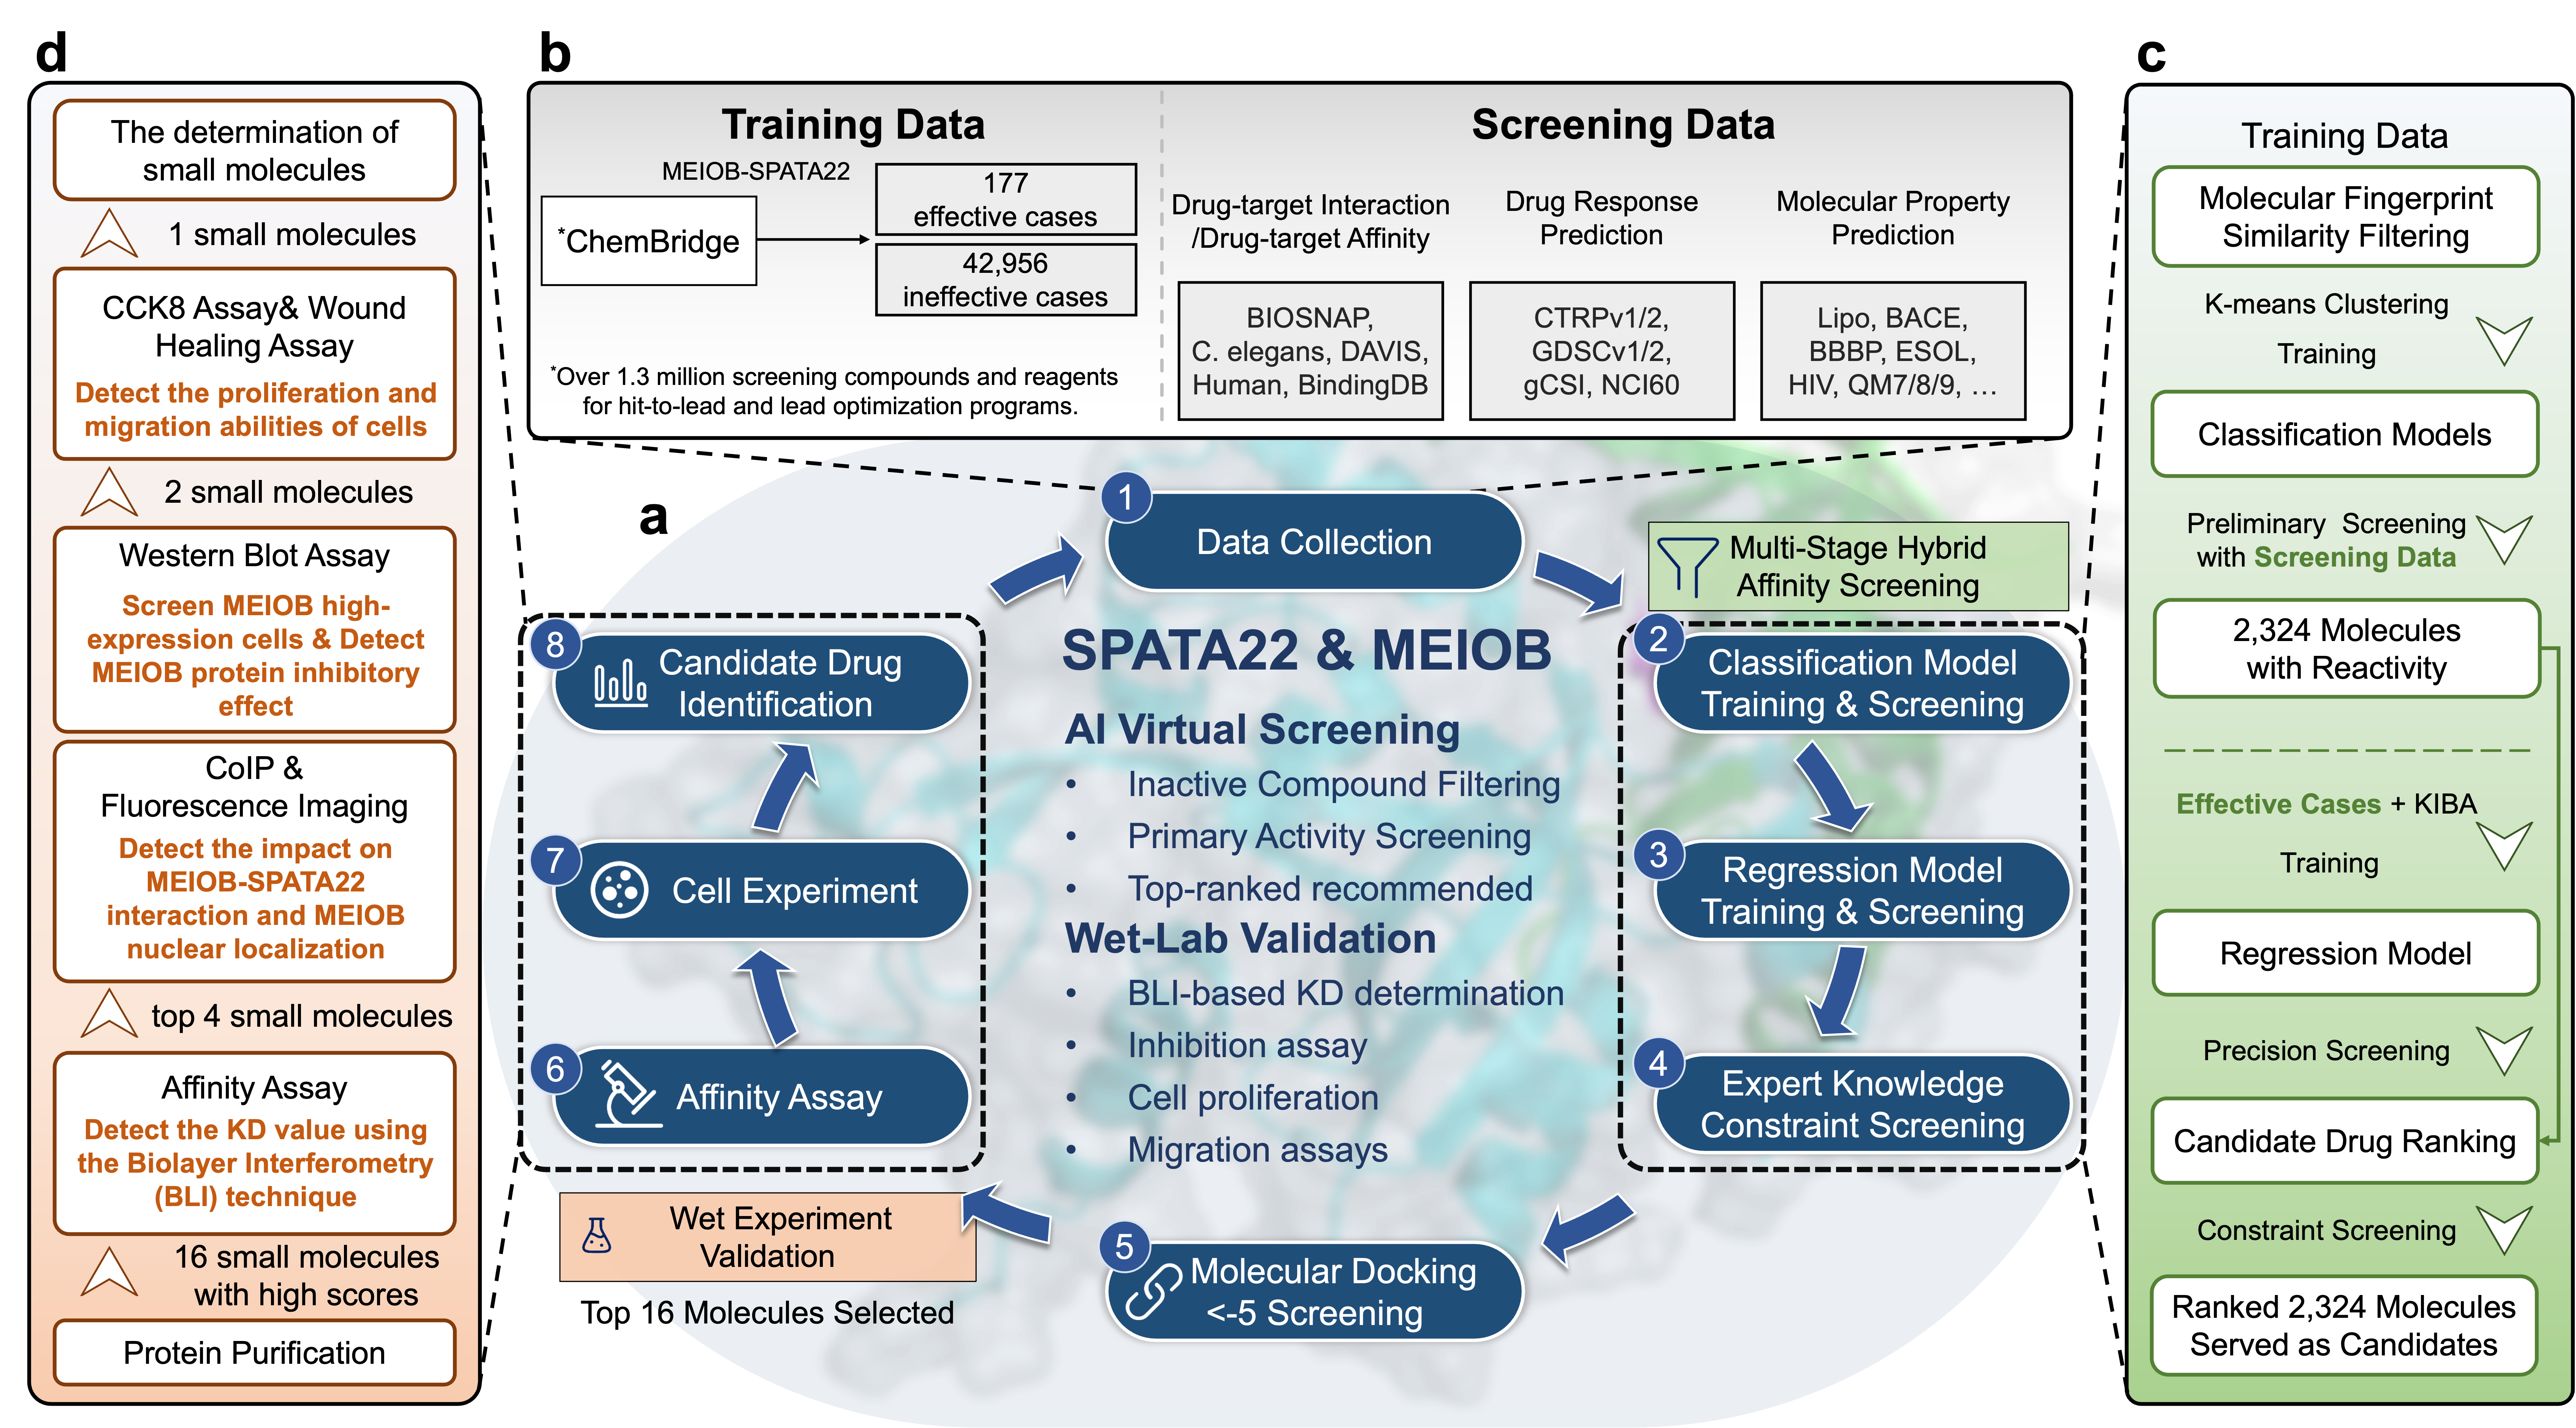
\includegraphics[width=0.8\linewidth]{pic/Fig 1.png}
    \caption{\textbf{Multi-stage hybrid screening solution for male contraceptives}. \textbf{a} Target-based multi-stage hierarchical screening solution for male contraceptive. The process includes target identification and validation, compound library preparation, virtual screening, and in vitro screening and evaluation at the cellular and molecular levels. \textbf{b} Preparation of the training and screening data. c The multi-stage hierarchical virtual screening workflow. \textbf{c} The multi-stage hierarchical virtual screening workflow. \textbf{d} In vivo evaluation, including protein purification, affinity assay, Co-Immunoprecipitation (Co-IP), cell fluorescence imaging, Western blot (WB), and cell function assays.}
    \label{fig:1}
\end{figure*}



Nevertheless, applying AI methods to drug screening of the MEIOB–SPATA22 complex still faces several practical challenges (\citealt{35,36}). The generalization ability of the models, depth of feature representation, and the complexity of the data impose significant constraints (\citealt{37}), and their performance is highly dependent on high-quality, balanced, and diverse training data (\citealt{38,39}). However, real-world biomedical data often suffer from incompleteness, bias, and noise, which severely undermine the accuracy and stability of model predictions (\citealt{40}). More critically, models that perform well on standardized benchmark datasets often fail to deliver satisfactory results in real-world compound screening, with a noticeable gap between theory and practice (\citealt{41}). In compound libraries containing millions of molecules, the proportion of active compounds is typically less than 0.1\%, and in extreme cases, it can be as low as 0.0001\% (\citealt{42,43}). This extreme class imbalance makes it difficult for models to effectively identify potential active molecules. Furthermore, proteins such as MEIOB, which are specific to the reproductive system, often have limited structural information and ligand-binding data in public databases, resulting in a lack of sufficient training samples for supervised learning models and presenting challenges related to distribution shift (\citealt{44}).


Therefore, this paper proposes a multi-stage, multi-model hybrid compound screening solution, termed \textbf{MMCDS}, targeting the key male contraceptive proteins MEIOB-SPATA22 (\citealt{9,15}). MMCDS integrates AI-driven molecule–protein affinity screening with wet-lab validation (Fig.~\ref{fig:1}). The molecular affinity screening comprises a two-stage large-scale molecular library screening followed by an affinity ranking stage using a regression-based model. The wet-lab evaluation consists of three sequential stages: affinity assay, cell experiment, and candidate drug identification. Based on the recommended results of the MMCDS solution, we performed systematic protein binding assays and cellular functional tests on the 16 molecules with the highest prediction scores, and successfully identified four lead compounds with significant clinical translational value. Their optimal equilibrium dissociation constant (KD) reaches 10$^{-7}$ M. Pyrogallol, the most potent small molecule identified, is hypothesized to exert inhibitory effects on MEIOB function through dual mechanisms: impeding its nuclear localization and reducing its expression levels. Furthermore, pyrogallol demonstrated the capacity to attenuate the proliferative and migratory potentials of cancer cells. Additionally, we collated and evaluated recent deep learning models under identical experimental conditions. Extensive virtual experiments validated the superiority of MMCDS over state-of-the-art (SOTA) methods for compound screening.  Our solution improved MSE, PCC, and SRCC on Davis by 4.8\%, 16.3\%, and 9.6\%, and on KIBA by 1.9\%, 7.3\%, and 2.2\%, demonstrating strong OOD generalization.

% Our solution improved key metrics on the Davis and KIBA datasets, achieving gains of 4.8\%/16.3\%/9.6\% and 1.9\%/7.3\%/2.2\% in mean squared error (MSE), Pearson correlation coefficient (PCC) (\citealt{45}), and Spearman's rank correlation coefficient (SRCC) (\citealt{46}), respectively. These results demonstrate robust out-of-distribution (OOD) generalization capabilities.


\begin{figure*}[ht!]
    \centering
    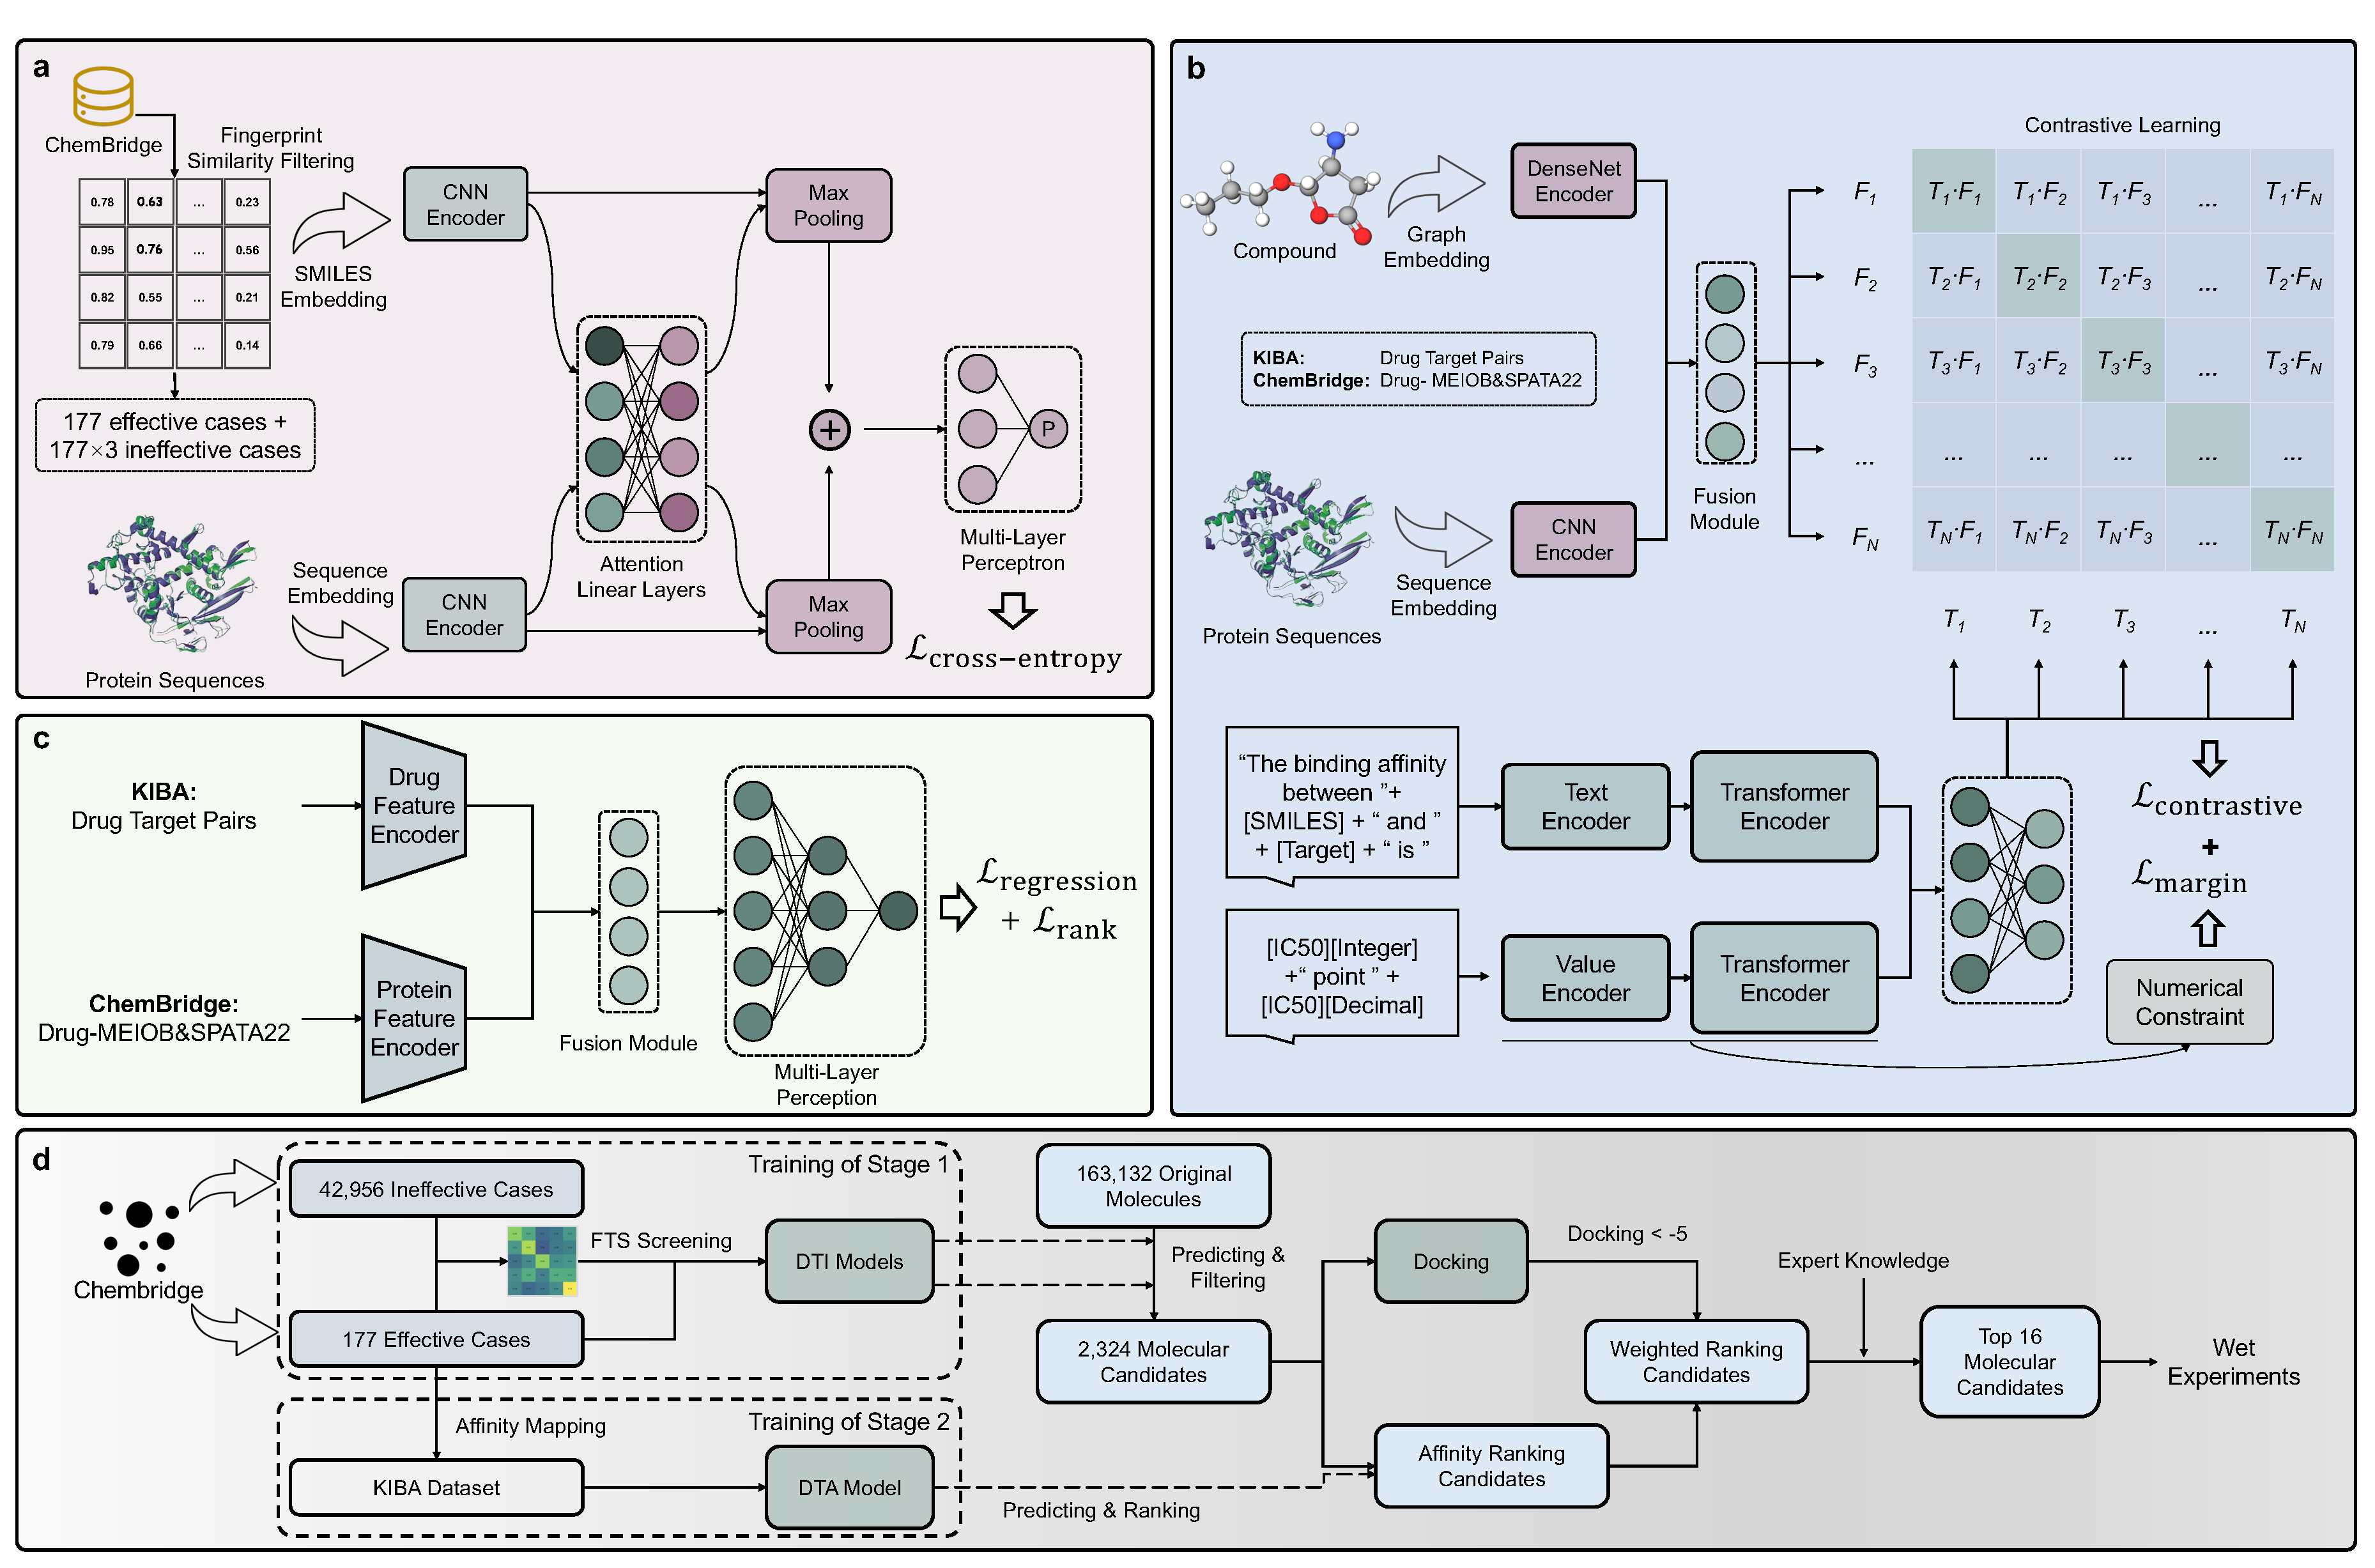
\includegraphics[width=0.9\linewidth]{newpic/fig_methods.pdf}
    \caption{\textbf{The model architectures used in each stage of MMCDS for the DTI/DTA tasks}. \textbf{a} Classification Stage selects ineffective cases closest to the effective ones according to fingerprint similarity filtering (FTS). Then it takes SMILES strings of drugs and sequences of MEIOB \& SPATA22 as input to predict their binding conditions. \textbf{b} The pre-training of the regression stage obtains the embedding of drugs' SMILES strings and protein sequences, as well as the textual description features of their interaction descriptions, aiming to predict the correct sample pairs through contrastive learning. \textbf{c} The fine-tuning of the regression stage uses the drug feature encoder and protein feature encoder in the pre-training stage. After fusing their features, the final multi-layer perception outputs their binding affinity. \textbf{d} Pipeline of utilizing our two models to predict and filter molecular candidates. Integrating with Schrödinger rigid docking and expert knowledge, 300 ultimate candidates were selected from 163,132 original molecules.}
    \label{fig:2}
\end{figure*}


\section*{Materials and methods}

\subsection*{Datasets and Metrics}

We use the 177 effective and 42,956 ineffective compounds derived from a previously reported cell-based high-content screen for the MEIOB-SPATA22 interaction (\citealt{67}) to train and test our drug-target interaction (DTI) models.
We also conducted out drug-target affinity (DTA) experiments on Davis (\citealt{52}) and KIBA (\citealt{53}) datasets, which are the most widely used datasets in DTA research.
The initial pool of candidate molecules is composed of widely used datasets from DTI, DTA, drug response prediction (DRP) and molecular property prediction (MPP), as these molecules are synthetic, non-toxic, and potentially suitable for pharmaceutical applications.
We further perform virtual molecular docking using Schrödinger on five potential pockets of MEIOB-SPATA22 to assist in evaluating the binding affinity of candidate molecules to the target.

For DTI models, we use accuracy score to evaluate the overall classification performance and recall score to measure the ability to recover true effective pairs.
For DTA models, we use mean squared error (MSE) to measure the deviation between predicted and true binding affinities, and we further use Pearson correlation coefficient (PCC) and Spearman rank correlation coefficient (SRCC) to assess the linear correlation and rank consistency between predictions and ground-truth values, and Rank score (\citealt{47}) to evaluate the model’s ability to prioritize high-affinity candidates.



\subsection*{MMCDS's framework}

To address the key challenges that impair real-world AI-driven drug screening, such as poor data quality, extreme class imbalance, and scarce information on male contraceptive targets, we have designed a multi-stage, multi-model hybrid screening solution named MMCDS. This solution is explicitly structured into two core computational stages to systematically evaluate and prioritize potential candidates for non-hormonal male contraceptives (Fig.~\ref{fig:1}). The first stage focuses on screening potential compounds in large-scale data. Since a single classification model cannot simultaneously filter out inactive molecules and extract active ones accurately, we apply two different training strategies to the same DTI model. These strategies effectively enable large-scale elimination of inactive molecules and maximize the recall of potential active molecules. The second stage then focuses on affinity prediction and ranking, where a DTA model is utilized to perform precise binding affinity predictions for the filtered candidates. These molecules are then ranked based on their predicted affinity to efficiently identify high-potential lead compounds.



\subsection*{Hierarchical Screening with Hard-negative Refinement} 

% In the classification task, we adopt a coarse-to-fine training strategy to enhance the identification of active compounds. Molecules exhibiting strong binding affinity to the target protein are treated as positive samples, whereas those with weak affinity are considered negative samples. The coarse screening phase is designed to efficiently eliminate a large proportion of irrelevant (negative) samples, while the fine screening phase focuses on accurately retrieving the true active compounds. Notably, the same classification model is employed in both phases, with differences only in the composition of the training data.

% In the coarse screening phase, a dataset is constructed by combining the positive samples with the top $k$ negative samples selected based on fingerprint similarity, which is then divided into validation and test sets. In the fine screening phase, we further account for the fact that certain positive samples, despite binding to the target protein, may lack actual inhibitory activity. Based on the empirical distribution of binding values, a threshold of $-4.2$ is established to distinguish true positive samples from false positives. The false positive samples, together with the top k negative samples, constitute the training and validation sets, while the true positive samples are reserved exclusively for testing the model performance.


We adopt a coarse-to-fine screening strategy to address severe class imbalance and the discrepancy between binding signals and true inhibitory activity. A single-stage classifier is easily dominated by abundant inactive molecules and therefore tends to learn only a coarse decision boundary.

In the coarse screening stage, molecules with strong binding affinity are treated as positive samples, whereas molecules with weak affinity are treated as negative samples. To mitigate the severe class imbalance, the negative set is constructed from the top-$k$ molecules with the highest fingerprint similarity to the positive samples. This strategy keeps the training set compact while retaining the most informative negatives, helping the model capture subtle structure--activity differences and achieve high-recall preliminary filtering. In the fine screening stage, we further separate likely active compounds from weakly binding-associated samples using a threshold of $-4.2$ derived from the empirical distribution of binding values. These ambiguous samples, together with the top-$k$ negatives, form a more challenging dataset for fine-grained discrimination, thereby refining the decision boundary toward true active compounds.


The model takes the SMILES sequence of a drug $S_d$ and the amino acid sequence of a target protein $S_p$ as input. They are encoded into latent representations $\mathbf{H}_d$ and $\mathbf{H}_p$ through embedding layers. The two representations are then integrated by a fusion module to obtain a joint feature vector $\mathbf{h}$, which is finally fed into a multi-layer perceptron to produce the prediction score $\hat{y}$:
\begin{equation}
\begin{aligned}
\mathbf{H}_d = \mathrm{Embedding}_d(S_d),& \quad
\mathbf{H}_p = \mathrm{Embedding}_p(S_p), \\
\mathbf{h} = \mathcal{F}_{\mathrm{fusion}}(\mathbf{H}_d, \mathbf{H}_p),& \quad \hat{y} = \mathrm{MLP}(\mathbf{h}).
\end{aligned}
\end{equation}

% The input to the model includes the SMILES sequence of the drug $S_{\text{drug}}$ and the amino acid sequence of the target protein $S_{\text{protein}}$. The drug features are extracted through an embedding layer $\text{Embedding}$, which can be formulated as:
% \begin{equation}
% \text{W}_{\text{drug}} = \text{Embedding}(S_{\text{drug}}),
% \end{equation}

% For protein feature extraction, the amino acid sequence is converted into a one-hot encoding or embedded via an embedding layer, generating protein features $F_{\text{protein}}$ as follows:
% \begin{equation}
% \text{W}_{\text{protein}} = \text{Embedding}(S_{\text{protein}}),
% \end{equation}

% The extracted drug features $\text{W}_{\text{drug}}$ and protein features $\text{W}_{\text{protein}}$ are subsequently used for feature fusion.

% An attention mechanism layer $ \mathcal{F}_ \text{attn}(\cdot)$ is employed to integrate the feature representations $(\text{W}_{\text{drug}}, \text{W}_{\text{protein}})$, and the fused feature matrix $\text{W}_{\text{fusion}}$ is obtained as follows:
% \begin{align}
% &\text{W}^{\text{drug}}_{\text{fusion}}  =   \mathcal{P}  \left( \left| \mathcal{F}_ \text{attn}(\text{W}_{\text{drug}}), \text{W}_{\text{drug}} \right| \right), \\
% &\text{W}^{\text{protein}}_{\text{fusion}}  =  \mathcal{P} \left( \left| \mathcal{F}_ \text{attn}(\text{W}_{\text{protein}}), \text{W}_{\text{protein}} \right| \right), \\
% &\text{W}_{\text{fusion}}  =  \mathcal{F}_ \text{attn} \left( \left| \text{W}^{\text{drug}}_{\text{fusion}}, \text{W}^{\text{protein}}_{\text{fusion}} \right| \right),
% \end{align}

% \noindent where, $\mathcal{P}(\cdot)$ denotes the max pooling operation, and $\left| \cdot \right|$ represents matrix concatenation. Finally, the fused features are passed through a multi-layer perceptron $\text{MLP}(\cdot)$ for prediction. The MLP is defined as:
% \begin{align}
% \hat{y} &= \text{MLP}(\text{W}_{\text{fusion}})\\
%  &= f^{(L)} \left( \cdots f^{(2)}(f^{(1)}(\text{W}_{\text{fusion}})) \right),
% \end{align}
% \noindent where $f^{(l)}$ represents the transformation in the $l$-th layer, typically consisting of a linear transformation followed by a non-linear activation function such as ReLU.

Let $y$ denote the ground truth labels and $\hat{y}$ the predicted outputs. The model is trained via cross-entropy loss function, defined as:
\begin{equation}
L(y, \hat{y}) = -\frac{\sum_{i=1}^{N} \left[ y_i \log(\hat{y}_i) + (1 - y_i) \log(1 - \hat{y}_i) \right]}{N}.
\end{equation}




\subsection*{Text-guided Affinity Ranking with Contrastive Learning}

After the coarse-to-fine screening stage, the remaining candidates are further prioritized by predicted binding affinity, and the top $N$ molecules are selected as the final recommendations. Since the MEIOB-SPATA22 complex involves only two target sequences, directly training an affinity predictor on the target-specific data may lead to limited representation diversity and weak generalization. To address this issue, we adopt a pre-training and fine-tuning strategy for affinity ranking. In the pre-training stage, drug-protein structural representations are aligned with natural language descriptions of their interactions through contrastive learning, enabling the model to capture transferable semantics beyond the narrow target space. In the fine-tuning stage, the structural encoder is optimized for affinity prediction, and a ranking objective is further introduced to improve the relative ordering of candidate molecules.

% For each drug-protein pair, the drug is encoded by a GCN, and the protein sequence is encoded by a 1D-CNN, and the resulting features are fused into a joint representation for downstream prediction. The interaction text is encoded by a Transformer to provide language supervision during pre-training. The model is first trained with a contrastive objective to align matched structure--text pairs in the shared embedding space, and is then fine-tuned using both mean squared error and ranking loss to predict binding affinity more accurately. This design enables the model to combine transferable representation learning with target-specific affinity ranking.


\begin{figure*}[ht!]
    \centering
    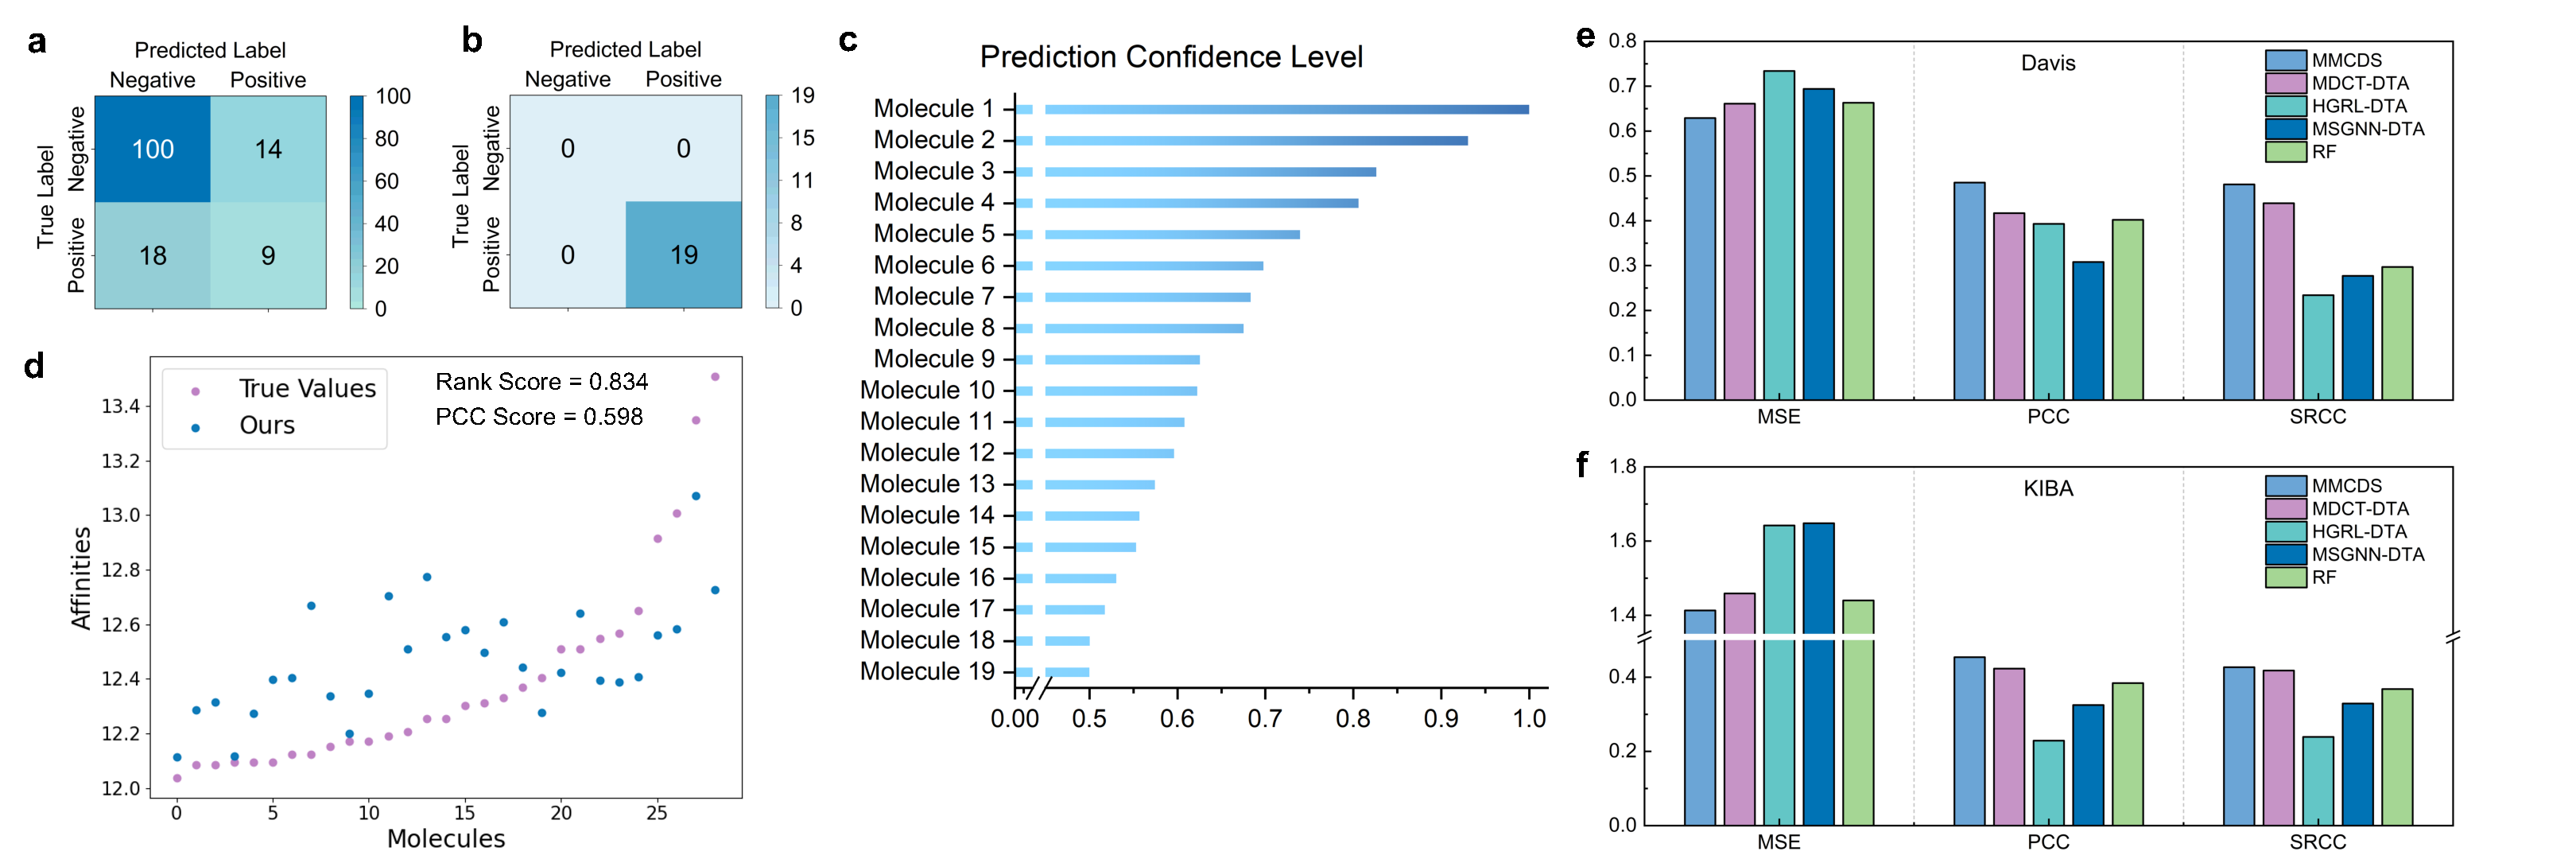
\includegraphics[width=0.9\linewidth]{newpic/fig2.pdf}
    \caption{\textbf{MMCDS's test results during the classification screening and regression ranking stages}. \textbf{a,b} Confusion matrices for the two training strategies in the initial classification stage: \textbf{a} focuses on filtering out a large number of inactive molecules, while \textbf{b} aims to retain potential active molecules. c Prediction confidence level of 19 test molecules in the first stage. \textbf{d} Comparison of predicted affinities by DTA model and true labels in the second stage. \textbf{e, f} OOD performance comparison of the DTA model against representative baseline methods on the Davis and KIBA datasets.}
    \label{fig:3}
\end{figure*}


We design a natural language-supervised contrastive learning framework during the pre-training phase (Fig.~\ref{fig:2}b). Specifically, for each input drug and protein pair $(\text{drug},\text{protein})$, the drug molecule is encoded using a multi-layer graph convolutional network (GCN) with dense connections to enhance atomic-level information flow, thereby capturing both local and global features. Their features are fused into a joint representation $\mathbf{F}$:
\begin{equation}
\mathbf{F} = \mathbf{W}_2 \, \mathrm{ReLU}\!\left(\mathbf{W}_1[\mathbf{H}_d;\mathbf{H}_p]\right),
\end{equation}
where $\mathbf{H}_d$ and $\mathbf{H}_p$ denote the encoded drug and protein features, respectively, and $[\cdot;\cdot]$ denotes feature concatenation.

To provide semantic supervision beyond the narrow target space, the natural language description associated with each drug--protein pair is encoded by a Transformer encoder to obtain a textual representation $\mathbf{T}$. We then use a contrastive objective to align matched structure--text pairs in the shared embedding space. Let
\begin{equation}
s_{ij} = \mathrm{sim}(\mathbf{F}_i,\mathbf{T}_j)
\end{equation}
denote the similarity between the $i$-th structural representation and the $j$-th textual representation. The contrastive loss is defined as
\begin{equation}
\mathcal{L}_{\mathrm{con}} =
-\frac{1}{N}\sum_{i=1}^{N}
\log
\frac{\exp(s_{ii}/\tau)}
{\sum_{j=1}^{N}\exp(s_{ij}/\tau)},
\end{equation}
where $\tau$ is the temperature parameter and $N$ is the batch size.

Besides semantic alignment, we further consider that textual descriptions often contain numerical information related to interaction strength or ordered relations, which cannot be fully captured by standard text encoding alone. To preserve such ordinal information, we transform the numerical text features into structured relational representations and introduce a margin-based objective inspired by knowledge graph modeling. Specifically, for each triplet $(h,l,t)\in\mathcal{S}$, where $h,t\in\mathcal{E}$ denote entities and $l\in\mathcal{L}$ denotes a relation, the margin loss is defined as
\begin{equation}
\mathcal{L}_{\mathrm{margin}}
=
\sum_{(h,l,t)\in\mathcal{S}}
\left[
\gamma + d(\mathbf{h}+\mathbf{l},\mathbf{t}) - d(\mathbf{t}+\mathbf{l},\mathbf{h})
\right]_+,
\end{equation}
where $[x]_+=\max(0,x)$, $\gamma>0$ is the margin parameter, and $d(\cdot,\cdot)$ denotes the distance function. In this way, numerical order information in the text branch is explicitly regularized and can complement the semantic alignment learned by contrastive pre-training.

The overall pre-training objective is therefore written as
\begin{equation}
\mathcal{L}_{\mathrm{pre}}
=
\mathcal{L}_{\mathrm{con}} + \mathcal{L}_{\mathrm{margin}}.
\end{equation}

In the fine-tuning stage, the pre-trained structural branch is retained for affinity prediction. The fused representation $\mathbf{F}$ is fed into an MLP regressor to predict the binding affinity $\hat{y}=\mathrm{MLP}(\mathbf{F})$. To improve both numerical accuracy and relative ranking quality, we jointly optimize the model with a mean squared error loss and a ranking loss:
\begin{align}
\mathcal{L}_{\mathrm{mse}} &=
\frac{1}{N}\sum_{i=1}^{N}(\hat{y}_i-y_i)^2, \\
\mathcal{L}_{\mathrm{rank}} &=
\sum_{i<j}
\max\!\left(0,\,-\mathrm{sign}(y_i-y_j)(\hat{y}_i-\hat{y}_j)\right),
\end{align}
The final fine-tuning objective is
\begin{equation}
\mathcal{L}_{\mathrm{fine}}
=
\mathcal{L}_{\mathrm{mse}} + \lambda\,\mathcal{L}_{\mathrm{rank}}.
\end{equation}
where $\lambda$ controls the contribution of the ranking term.

% Through this design, the model first learns transferable drug--target representations by aligning structural features with textual semantics and numerical order information, and then adapts these representations to target-specific affinity prediction and candidate prioritization.

% $L$-layer GCN is defined as:
% \begin{equation}
%     \mathbf{H}^{(l+1)} = \sigma\left( \tilde{D}^{-\frac{1}{2}}\tilde{A}\tilde{D}^{-\frac{1}{2}}\mathbf{H}^{(l)}\mathbf{W}^{(l)} \right),
% \end{equation}
% where, $\tilde{A} = A + I$ (adjacency matrix with self-loops), $\tilde{D}$ is its degree matrix, $\mathbf{W}^{(l)}$ learnable weights, and $l \in [0,...,L-1]$. The protein sequence is processed via a one-dimensional CNN, denoted as:
% \begin{equation*}
%     \mathbf{P}^{(l+1)} = \text{ReLU}\left( \text{Conv1D}(\mathbf{P}^{(l)}, \mathbf{K}^{(l)}) \right)
% \end{equation*}
% where, $\mathbf{K}^{(l)}$ denoting convolution kernels. Let $\text{W}_{\text{drug}}$ and $\text{W}_{\text{protein}}$ denote the extracted representations of the drug and protein, respectively. These features are then fused by the MLP to obtain a joint representation $\mathbf{F}$ for subsequent tasks.
% \begin{align}
% \mathbf{F} = \mathbf{W}_2 \text{ReLU}(\mathbf{W}_1 [\text{W}_{\text{drug}}; \text{W}_{\text{protein}}])
% \end{align}
% where, $\mathbf{W}_1 \in \mathbb{R}^{d_h \times (d_d + d_p)}$ is first layer weights, $\mathbf{W}_2 \in \mathbb{R}^{d_f \times d_h}$
% is second layer weights, and $[\cdot;\cdot]$ is concatenation operator. Then, the natural language description $\text{T}_\text{desc}$ of each sample is encoded by a Transformer encoder to obtain the textual embedding $\mathbf{T}$:
% \begin{align}
% \mathbf{H} &= \text{LayerNorm}(\text{T}_\text{desc} + \text{MHA}(\text{T}_\text{desc})),\\
% \mathbf{T} &= \text{TransformerBlock}(\text{T}_\text{desc}) \\ \nonumber
% &= \text{LayerNorm}(\mathbf{H} + \text{FFN}(\mathbf{H})),
% \end{align}
% where, $\text{MHA}(\cdot)$ is multi-head attention and $\text{FFN}(\cdot)$ is a position-wise feed-forward network. We adopt a contrastive learning objective to align the matching pairs $(F_i, T_i)$ in the embedding space. Specifically, let $s_{ij} = \text{sim}(F_i, T_j)$ denote the cosine similarity between the $i$-th structure pair and the $j$-th textual description. The training objective encourages the diagonal elements $s_{ii}$ to be the highest in their rows and columns. The contrastive loss is formulated as:
% \begin{equation}
% \mathcal{L}_\text{contrastive} = - \frac{1}{N} \sum_{i=1}^{N} \log \frac{\exp(s_{ii} / \tau)}{\sum_{j=1}^{N} \exp(s_{ij} / \tau)}
% \end{equation}
% where $\tau$ is the temperature parameter, and $N$ is the batch size. When dealing with numerical information, we must consider incorporating numerical features into the model to represent their relationships more accurately. To enhance the value encoder's efficiency in capturing numerical relationships, we employ a margin-based loss function $\mathcal{L}_\text{margin}$. The objective is to minimize the distance between entity embeddings for pairs satisfying the relationship while maximizing it for negative pairs:
% \begin{equation}
% \mathcal{L}_\text{margin} = \sum_{(h,l,t) \in \mathcal{S}} \left[ \gamma + d(\mathbf{h} + \mathbf{l}, \mathbf{t}) - d(\mathbf{t} + \mathbf{l}, \mathbf{h}) \right]_+
% \end{equation}
% where $[x]_+ = \max(0,x)$, $\gamma > 0$ is a margin hyperparameter, and $\mathcal{S}$ consists of triplets $(h,l,t)$ with $h,t \in \mathcal{E}$ and $l \in \mathcal{L}$. The embeddings $\mathbf{h}, \mathbf{l}, \mathbf{t} \in \mathbb{R}^k$ (where $k$ is the embedding dimension) are learned parameters. The distance function $d(\cdot,\cdot)$ can be either $L_1$ or $L_2$ norm. Numerical relationships are regularized by $\mathcal{L}_{\text{margin}}$ in the number encoder $\Phi_{\text{number}}(T_{\text{number}}(\mathcal{E}))$. Each relationship $l$ is represented as a learnable embedding vector.


% Therefore, the total loss function during pre-training is formulated as the combination of both objectives:
% \begin{equation}
% \mathcal{L}_\text{pre-training} = \mathcal{L}_\text{margin} + \mathcal{L}_\text{contrastive}
% \end{equation}


% % \subsection*{Fine-tuning} 
% In the fine-tuning stage (Fig.~\ref{fig:2}c), we retain the structure branch to perform regression tasks. The fused representation $\mathbf{F}$ is fed into a Multi-Layer Perceptron (MLP) regressor to predict a scalar value $\hat{y}_i$, aiming to approximate the ground-truth label $y_i$. 
% \begin{align}
% \hat{y} = \text{MLP}(\mathbf{F}; \{\mathbf{W}_\ell, \mathbf{b}_\ell\}_{\ell=1}^L)
% \end{align}
% where, $\mathbf{W}_\ell \in \mathbb{R}^{d_\ell \times d_{\ell-1}}$ are weight matrices for layer $\ell$, and $\mathbf{b}_\ell \in \mathbb{R}^{d_\ell}$ are bias terms. Additionally, to account for noise and potential errors introduced during data mapping, we incorporate a ranking loss function alongside the standard regression loss to better capture the relative order of predicted affinities. 

% During the fine-tuning stage, we optimize the model using both MSE and ranking loss:
% \begin{align}
% \mathcal{L}_\text{mse} & = \frac{1}{N} \sum_{i = 1}^{N} (\hat{y}_i - y_i)^2 \\
% \mathcal{L}_\text{rank} & = \sum_{i < j} \max\left(0, -\text{sign}(y_i - y_j)(\hat{y}_i - \hat{y}_j)\right)
% \end{align}

% Finally, the total fine-tuning loss is
% $\mathcal{L}_\text{fine-tuning} = \mathcal{L}_\text{regression} +  \mathcal{L}_\text{rank}$.


% Through these steps, MMCDS effectively integrates classification and regression stages, significantly enhancing screening efficiency and providing crucial support for the precise selection of drug candidates. This novel model not only offers a new direction for the development of male contraceptives but also lays the groundwork for drug discovery in other fields.




\begin{figure*}[ht!]
    \centering
    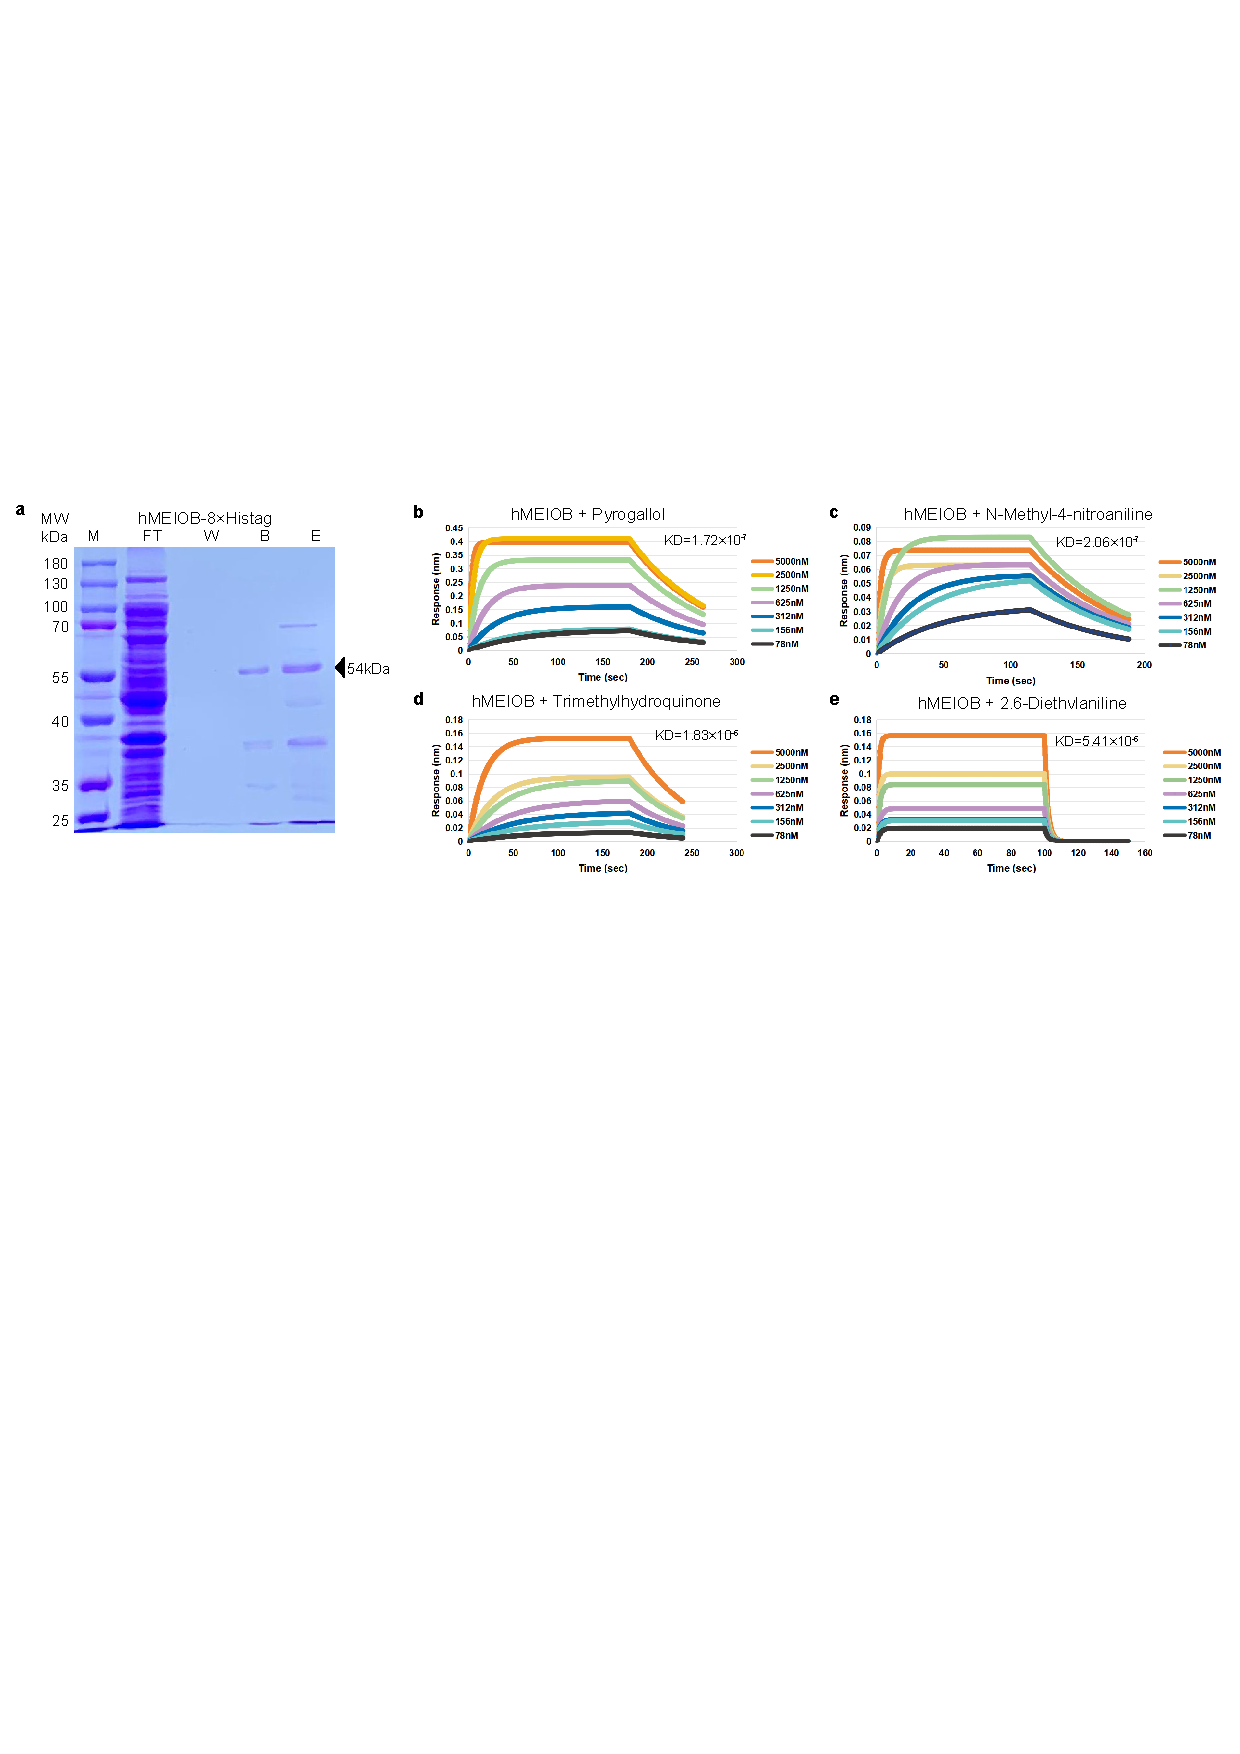
\includegraphics[width=0.9\linewidth]{newpic/fig3-.pdf}
    % \caption{\textbf{Affinity detection of small molecules for MEIOB}. \textbf{a} Purify the full-length human MEIOB-8×His-Tag protein from E. coli using Ni-NTA beads. M: Markers; FT: Flow-through; W: Wash; b: Beads; E: Elution. \textbf{b} Fitting curve of Pyrogallol and MEIOB. \textbf{c} Fitting curve of N-Methyl-4-nitroanilinel and MEIOB. \textbf{d} Fitting curve of trimethylhydroquinonel and MEIOB.  \textbf{e} Fitting curve of 2,6-Diethylaniline and MEIOB. \textbf{f} Chemical Structures and $\text{KD}$ Values of candidates molecules with MEIOB, with overfitting observed in detection curves for several small molecules.}
    \caption{\textbf{Affinity detection of small molecules for MEIOB.} \textbf{a} Purify the full-length human MEIOB-8 × His-Tag protein from E. coli using Ni-NTA beads. M: Markers; FT: Flow-through; W: Wash; b: Beads; E: Elution. \textbf{b} Fitting curve of Pyrogallol and MEIOB. \textbf{c} Fitting curve of N-Methyl-4-nitroanilinel and MEIOB. \textbf{d} Fitting curve of trimethylhydroquinonel and MEIOB. \textbf{e} Fitting curve of 2,6-Diethylaniline and MEIOB.}
    \label{fig:4}
\end{figure*}



% \section*{Results}

\section*{Results}


\begin{figure*}[ht!]
    \centering
    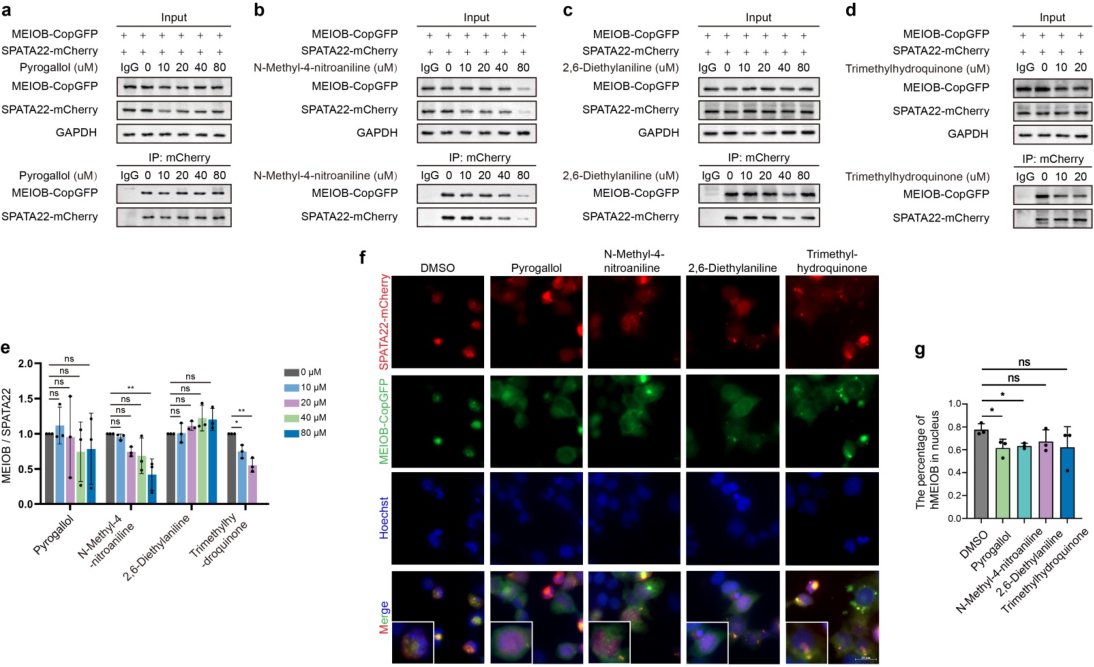
\includegraphics[width=0.9\linewidth]{newpic/fig4.pdf}
        % \caption{\textbf{Effect of Small Molecules on the Interaction between MEIOB and SPATA22}. \textbf{a-d} MEIOB-CopGFP expressing plasmid was co-transfected with SPATA22-mCherry expressing plasmid into HEK 293T cell, and co-incubated with candidate molecules at different concentrations for 48 h. mCherry IP experiment was conducted on the cell lysates. IgG IP was set as negative control. \textbf{e} Effects of candidate molecules at different concentrations on the interaction between MEIOB and SPATA22 in HEK 293T cells. Following IP of samples using the mCherry antibody, the ratio of the gray values of MEIOB protein to SPATA22 protein was determined, and normalization was performed using the ratio from the 0 $\mu$M candidate molecule group as a reference. All results were obtained from three independent replicates. All data were analyzed using the two-way ANOVA and presented as mean±SD ($^{\ast}P < 0.5$, $^{\ast\ast}P < 0.01$).}
        \caption{\textbf{Effect of Small  Molecules on the  Interaction between  MEIOB and SPATA22 and affect MEIOB nuclear localization.} \textbf{a}-\textbf{d}  MEIOB-CopGFP expressing plasmid was co-transfected with SPATA22-mCherry expressing plasmid into  HEK  293T  cell,  and co-incubated with candidate molecules at different concentrations for 48 h.  mCherry  IP experiment was conducted on the cell lysates. IgG IP was set as a negative control. \textbf{e} Effects of candidate molecules at different concentrations on the interaction between MEIOB and SPATA22 in HEK 293T cells. Following IP of samples using the mCherry antibody, the ratio of the gray values of MEIOB protein to SPATA22 protein was determined, and normalization was performed using the ratio from the 0 $\mu$M candidate molecule group as a reference. All results were obtained from three independent replicates. Data were analyzed using the two-way ANOVA and presented as mean±SD ($^\ast P < 0.5$, $^{\ast\ast} P < 0.01$). \textbf{f} The distribution of MEIOB-CopGFP (green), SPATA22-mCherry (red), and Hochset (blue) in HEK 293T cells. MEIOB-CopGFP expressing plasmid was co-transfected with SPATA22-mCherry expressing plasmid into HEK 293T cells, and co-incubated with candidate molecules at different concentrations for 48 h. Scale bar: 20 $\mu$m. \textbf{g} Statistical analysis of the distribution of MEIOB-CopGFP in the cytoplasm and nucleus of HEK 293T cells co-expressing MEIOB-CopGFP and SPATA22-mCherry. The experiment was repeated three times, with the localization of 100 cells counted each time; data were analyzed using the unpaired t-test and presented as mean$\pm$SD ($^\ast P < 0.5$).}
    \label{fig:5}
\end{figure*}





To systematically evaluate MMCDS, we organized the experimental study into two sequential parts: computational evaluation and biological validation. The computational part was designed to assess whether the proposed two-stage framework could accurately filter large-scale compound libraries and prioritize candidates with high binding potential toward the MEIOB-SPATA22 complex. The biological part was designed to verify whether the selected compounds truly bind MEIOB and whether they further affect the MEIOB-SPATA22 interaction and its downstream cellular phenotypes.



\subsection*{Computational Evaluation}

This section evaluates the effectiveness and state-of-the-art nature of the MMCDS method from the perspective of virtual screening. This part of the study is primarily divided into three levels. First, we evaluate the performance of the hierarchical screening stage, focusing on its ability to retain potential active compounds while removing invalid molecules. Second, we evaluate the performance of the affinity ranking stage, focusing on its generalization ability under out-of-distribution settings. Finally, we apply the complete computational workflow to screen large-scale molecular libraries and use the resulting candidate molecules for downstream wet-lab validation.

\subsubsection*{Large-scale high-precision compound filtering} % 分类模型的表现

In the first stage, the primary objective is to filter out molecules that do not exhibit significant interactions with the MEIOB-SPATA22 complex, a protein complex involved in the regulation of male fertility, while ensuring that potentially effective molecules are not overlooked. To achieve this, we designed a hybrid deep learning model that integrates attention mechanisms with CNNs to perform the DTI task. To address the limitations of existing datasets, we further developed and implemented two distinct versions of the model, each optimized for specific tasks within the screening process.

Specifically, the first training strategy aims to eliminate as many ineffective cases as possible while retaining the majority of effective ones. To achieve this, we selected the top three negative samples with the highest fingerprint similarity from ChemDiv and ChemBridge out of the 177 effective cases, which were then used to construct the training and testing sets. The second training strategy focuses on maximizing the model's ability to recall as many true effective cases as possible. Considering that the binding affinities of effective cases with MEIOB-SPATA22 vary, we classified the effective cases based on their distribution, dividing them into 19 true effective cases and 158 false effective cases, with a threshold of $-4.2$. In this case, the false-effective cases and the ineffective cases generated in the first stage were used to form the training and validation sets, while the true-effective cases were reserved for the testing set.

As illustrated in the first confusion matrix, the first training strategy achieves an accuracy score of 0.77, effectively eliminating a large proportion of ineffective cases while preserving a substantial fraction of positive candidates (Fig.~\ref{fig:2}a). Such a result demonstrates its robustness in distinguishing interacting from non-interacting compounds. Moreover, the second training strategy achieves a perfect recall score of 1.00 during the test phase (Fig.~\ref{fig:2}b). We present the prediction confidence level of all 19 test molecules (Fig.~\ref{fig:2}c). Not only are all 19 true effective cases sorted out, but 11 of them are also recalled with confidence greater than 0.6, exhibiting superior sensitivity. 




\begin{figure*}[ht!]
    \centering
    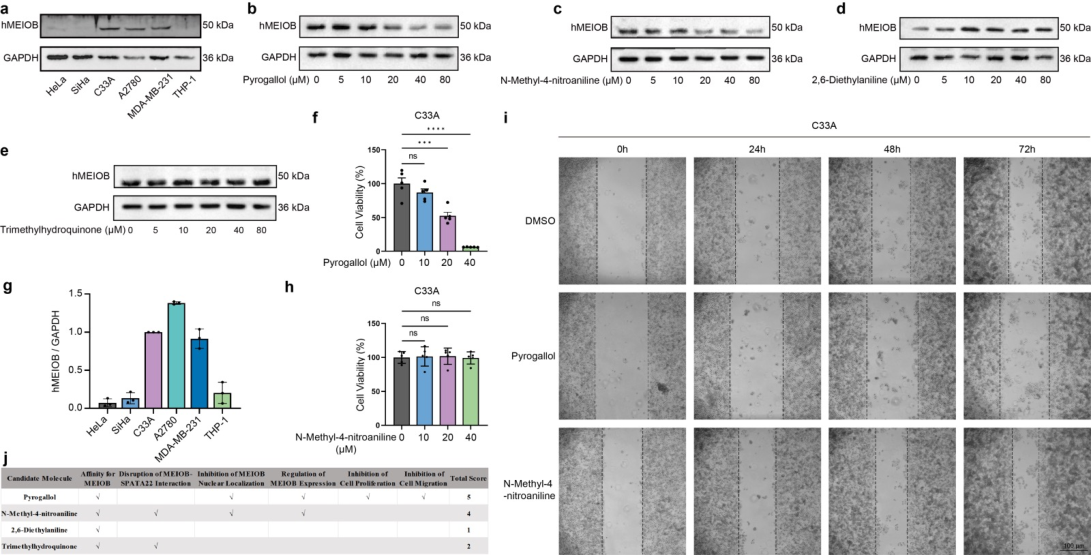
\includegraphics[width=0.9\linewidth]{newpic/fig5.pdf}
        % \caption{\textbf{Small molecules affect the nuclear localization of MEIOB}. \textbf{a} The distribution of MEIOB-CopGFP(green), SPATA22-mCherry(red), and Hochset (blue) in HEK 293T cells. MEIOB-CopGFP expressing plasmid was co-transfected with SPATA22-mCherry expressing plasmid into HEK 293T cell, and co-incubated with candidate molecules at different concentrations for 48 h. Scale bar: 20 $\mu$m. \textbf{b} Statistical analysis of the distribution of MEIOB-CopGFP in the cytoplasm and nucleus of HEK 293T cells co-expressing MEIOB-CopGFP and SPATA22-mCherry. The experiment was repeated three times, with the localization of 100 cells counted each time; all data were analyzed using the unpaired t-test and presented as mean±SD ($^{\ast}P < 0.5$).}
        \caption{\textbf{Small molecules inhibit MEIOB expression and cellular functions in C33A Cells.}  \textbf{a} Detect the expression of hMEIOB in various tumor cells  (HeLa,  SiHa,  C33A,  A2780,  MDA-MB-231,  THP-1).  \textbf{b} The expression level of hMEIOB in C33A cells after treatment with pyrogallol for 48 h. \textbf{c} The expression level of hMEIOB in C33A cells after treatment with N-methyl-4-nitroaniline for 48 h. \textbf{d} The expression level of hMEIOB in C33A cells after treatment with 2,6-diethylaniline for 48 h.  \textbf{e} The expression level of hMEIOB in C33A cells after treatment with trimethylhydroquinonel for 48 h.  \textbf{f} The cell viability of C33A cells after treatment with pyrogallol for 24 h. n=3/group, $^{\ast\ast\ast} P < 0.001$, $^{\ast\ast\ast\ast} P < 0.0001$, by two-way ANOVA. Experiments were independently repeated at least three times, and data are shown as the mean$\pm$SD.  \textbf{g}  Expression  levels  of hMEIOB  protein  in  different  tumor cell  lines(HeLa,  SiHa,  C33A,  A2780, MDA-MB-231, THP-1). Protein expression levels were quantified by gray values. The relative expression level of hMEIOB was normalized using GAPDH as an internal reference (expressed as the hMEIOB/GAPDH ratio), and then further normalized to the hMEIOB/GAPDH ratio of the C33A group in each experimental set. Band quantification was normalized to GAPDH. All experiments were independently repeated three times, and the quantitative results were presented as mean$\pm$SD.  \textbf{h} The cell viability of C33A cells after treatment with N-methyl-4-nitroanilinel for 24 h. n=3/group, and data were analyzed using the two-way ANOVA. All experiments were independently repeated at least three times, and data are shown as the mean±SD. \textbf{i} The wound-healing assay was employed to assess the impacts of pyrogallol and N-methyl-4-nitroaniline on the migratory capacity of C33A cells.  \textbf{j} Scoring of MEIOB-related assays for candidate molecules. Each positive result counted as 1 point.}
    \label{fig:6}
\end{figure*}




\subsubsection*{Affinity prediction and ranking} % 亲和度预测结果

Following the initial screening, the second stage of our solution focuses on predicting and ranking the binding affinities of the selected molecular candidates. This stage is crucial for refining the selection process and prioritizing compounds with the highest likelihood of effective interaction with MEIOB-SPATA22. Therefore, we proposed a dedicated DTA model, pre-trained under natural language supervision and fine-tuned by approaching regression values, to estimate the binding strengths, providing a quantitative assessment of molecular affinity.

To evaluate our DTA model's performance, we integrated 177 effective cases with specific affinities into KIBA, and randomly splited them into training and test sets. Notably, 29 effective cases were divided into the test set, and we provide a detailed visualization for testing analysis (Fig.~\ref{fig:2}d). The data distribution predicted by our DTA model is basically consistent with the true affinities of effective cases. Specifically, it achieves 0.834 in Rank score and 0.598 in PCC score, which reinforces the reliability of our model, as well as exhibits a more precise and biologically relevant ranking of candidate molecules. In practical applications, only a subset of top-ranked molecules is typically selected for experimental validation. A higher Rank score is particularly important in drug screening, as it reflects the model's ability to rank molecules based on predicted binding affinities.


Additionally, we conducted a comparative analysis of the DTA model of MMCDS against SOTA methods, including machine learning techniques such as random forest (RF) (\citealt{48,49}), and deep learning models like MSGNN-DTA (\citealt{50}), HGRL-DTA (\citealt{51}), and MDCT-DTA (\citealt{27}).
% We used three metrics to measure the performance of the model on regression tasks. MSE measures the mean square error between predicted and true values. The PCC measures the linear relationship between true values and predicted values. The SRCC considers level correlation without parameters, assuming that two sets of data are not sampled in a normal distribution.

Since our drug discovery process is a task for unseen drugs, which is an OOD problem, we designed the scenario where the drugs in the test set are absent from the training set for our experiment. In this way, we will effectively assess the OOD performance of different DTA models. MMCDS outperforms all comparative baseline models across all criteria on both Davis and KIBA datasets (Fig.~\ref{fig:2}e and Fig.~\ref{fig:2}f). Specifically, MMCDS achieved improvements of 4.8\%, 16.3\%, and 9.6\% in MSE, PCC, and SRCC, respectively, on the Davis dataset. Additionally, it demonstrated enhancements of 1.9\%, 7.3\%, and 2.2\% in MSE, PCC, and SRCC, respectively, on the KIBA dataset, showcasing its superior generalization capability for OOD problems.


\subsubsection*{Large-scale virtual screening and candidate prioritization}

Initially, by sequentially applying two different strategies to train the DTI models for filtering the initial pool of 163,132 small molecules, 2,324 molecular candidates demonstrating potential interactions with MEIOB-SPATA22 were successfully identified. Afterwards, our DTA model predicted the affinity scores of the 2,324 molecular candidates. We integrate predicted affinity scores with Schrödinger docking results to comprehensively evaluate each candidate. Based on this multifaceted assessment, these candidate molecules with the greatest potential were ultimately screened out. Finally, compounds with poor druggability were excluded, and 16 compounds that are currently readily accessible were selected for subsequent research. Our multi-stage, multi-model solution completes the stages of training, screening, prediction, and ranking within a few days, systematically evaluating and selecting potential drug candidates, demonstrating its significant potential in accelerating the discovery of novel therapeutics with high specificity and efficacy.

SPATA22 functions as a chaperone protein for MEIOB. The absence of SPATA22 gives rise to the ablation of MEIOB functionality (\citealt{6,9,10}). Previously, we have successfully tested the binding affinity between proteins and small molecules using biolayer interferometry (BLI) technology (\citealt{11}). Therefore, to screen for small molecules that are capable of engaging in true competitive binding to MEIOB against SPATA22, we expressed full-length soluble MEIOB and used 8×His-Tag as a fusion protein, which was used to bind to NTA biosensors to assess the affinity of candidate molecules, specifically the $\text{KD}$ value (Fig.~\ref{fig:4}a). The 16 screened candidate molecules were detected using BLI technology (Supplementary Table S1). After statistical analysis and removing the candidate molecules with overly fluctuating curves, the results showed that the $\text{KD}$ values of 4 candidate molecules binding to MEIOB reached the 10$^{-6}$M, including pyrogallol, N-methyl-4-nitroaniline, trimethylhydroquinone, and 2,6-diethylaniline. Among them, the $\text{KD}$ values of pyrogallol and N-methyl-4-nitroaniline reached 1.72×10$^{-7}$M and 2.06×10$^{-7}$M (Fig.~\ref{fig:4}b-e). These four candidate molecules specifically bind to MEIOB.

To investigate the action sites through which these candidate molecules interfere with the interaction between MEIOB and SPATA22, we predicted the structures of MEIOB (aa272-471) and SPATA22 (aa236-363) and constructed computational models of these candidate molecules binding to the complex. The model showed that pyrogallol inserts into the pocket of the MEIOB-SPATA22 complex and interacts with the SER 462 residue of MEIOB via hydrogen bonding; N-methyl-4-nitroaniline interacts with the SER 462, SER 466, and ARG 429 residues of MEIOB; 2,6-diethylaniline associates with the SER 462 and SER 466 residues of MEIOB; and trimethylhydroquinone acts on the SER 466 and ARG 429 sites of MEIOB (Supplementary  Fig. S1). Collectively, BLI assays and molecular docking experiments confirmed that the four lead compounds exhibit high-affinity binding to MEIOB, with distinct binding sites mapped at key residues (e.g., SER 462, SER 466, ARG 429) within the MEIOB-SPATA22 interaction interface. These results not only validate the specific binding capacity of the identified compounds but also underscore the reliability and predictive power of MMCDS in screening high-potential lead molecules.



\subsection*{Biological Validation}


We then performed biological validation to determine whether the computationally selected candidates exert measurable effects on MEIOB and its interaction with SPATA22. This section includes validation of interaction disruption, assessment of MEIOB nuclear localization, evaluation of MEIOB expression in C33A cells, and examination of downstream cellular phenotypes such as proliferation and migration.


\subsubsection*{N-Methyl-4-nitroaniline and Trimethylhydroquinone Inhibits MEIOB-SPATA22 Interaction}

MEIOB interacts with SPATA22, and the aa294-450 region of MEIOB serves as the binding domain for SPATA22. During meiosis, MEIOB can only be recruited to DNA double-strand breaks (DSBs) sites to exert its normal function in the presence of SPATA22 (\citealt{1,2}). To investigate whether the candidate molecules could disrupt the interaction between MEIOB and SPATA22, we co-transfected CopGFP-tagged MEIOB and mCherry-tagged SPATA22 in cells and treated them with different concentrations of candidates (pyrogallol, N-methyl-4-nitroaniline, trimethylhydroquinone, and 2,6-diethylaniline) for detection. Results showed that after treatment with trimethylhydroquinone at concentrations of 10 $\mu$M and 20 $\mu$M (note: high concentrations of trimethylhydroquinone exhibited relatively strong cytotoxicity), the level of MEIOB bound to SPATA22 decreased with increasing drug concentration (Fig.~\ref{fig:5}d,e). Similar results were observed in cells treated with N-methyl-4-nitroaniline (Fig.~\ref{fig:5}b,e). However, no obvious effect was detected following treatment with pyrogallol or 2,6-diethylaniline (Fig.~\ref{fig:5}a,c,e). Collectively, these findings indicate that trimethylhydroquinone and N-methyl-4-nitroaniline can disrupt the interaction between MEIOB and SPATA22.




\subsubsection*{Pyrogallol and N-Methyl-4-nitroaniline Affect MEIOB Nuclear Localization}

In the presence of SPATA22, MEIOB translocates into the nucleus, and the two proteins localize at DSBs sites to exert repair functions. When SPATA22 is absent in cells or the interaction between the two is disrupted, MEIOB cannot expose its nuclear localization signal (NLS) to enter the nucleus (\citealt{10}). To investigate whether candidates affect the nuclear localization of MEIOB, we co-transfected CopGFP-MEIOB and mCherry-SPATA22, and observed the localization of MEIOB and SPATA22 after candidate treatment. Imaging and statistical results showed that in the absence of candidates, MEIOB co-localized with SPATA22 in the nucleus. After treatment with pyrogallol and N-methyl-4-nitroaniline, the nuclear localization of MEIOB decreased, and it was instead expressed in the cytoplasm. However, no significant change in the nuclear localization of MEIOB was observed after treatment with 2,6-diethylaniline and trimethylhydroquinone (Fig.~\ref{fig:5}f,g). Collectively, cell fluorescence imaging and statistical analyses demonstrated that pyrogallol and N-methyl-4-nitroaniline specifically disrupt the nuclear localization of MEIOB, whereas 2,6-diethylaniline and trimethylhydroquinone exert no significant effect on the subcellular localization of MEIOB. These findings confirm that specific candidate molecules can interfere with the nuclear translocation of MEIOB, likely by disrupting the interaction between MEIOB and SPATA22.


\subsubsection*{Pyrogallol and N-Methyl-4-nitroaniline Inhibit the Expression of MEIOB in C33A Cells}

Previous studies have found that MEIOB is involved in the repair of DSBs during meiotic homologous recombination. It not only participates in the regulation of spermatogenesis but also, as a cancer-testis gene, regulates the occurrence and development of diseases in tumors such as breast cancer, lung adenocarcinoma, and melanoma, showing a tumor-promoting effect (\citealt{18,19,20}). Therefore, we intend to test the potential of candidate molecules for cancer therapy in subsequent studies. First, we screened out several cell lines that may highly express MEIOB through the Human Protein Atlas (HPA) database (\url{https://www.proteinatlas.org/}) and confirmed by WB that MEIOB was highly expressed in the cervical cancer cell line C33A, ovarian cancer cell line A2780, and breast cancer cell line MDA-MB-231. Among these cell lines, A2780 exhibited the highest MEIOB expression level, followed by C33A and MDA-MB-231 (Fig.~\ref{fig:6}a,g). However, due to the relatively low incidence rate of ovarian cancer, we selected the cervical cancer cell line C33A, which has high expression of MEIOB and a high incidence rate, for validation in subsequent experiments.

Next, we treated C33A cells with pyrogallol, N-methyl-4-nitroaniline, 2,6-diethylaniline, and trimethylhydroquinone. It was found that after treatment with pyrogallol or N-methyl-4-nitroaniline for 48 h, the protein level of MEIOB in the cells was down - regulated with the increase in the concentration of the small molecule, showing an inhibitory effect on MEIOB (Fig.~\ref{fig:6}b,c). 2,6-Diethylaniline and trimethylhydroquinone had no inhibitory effect on MEIOB (Fig.~\ref{fig:6}d,e).

% \begin{figure*}
%     \centering
%     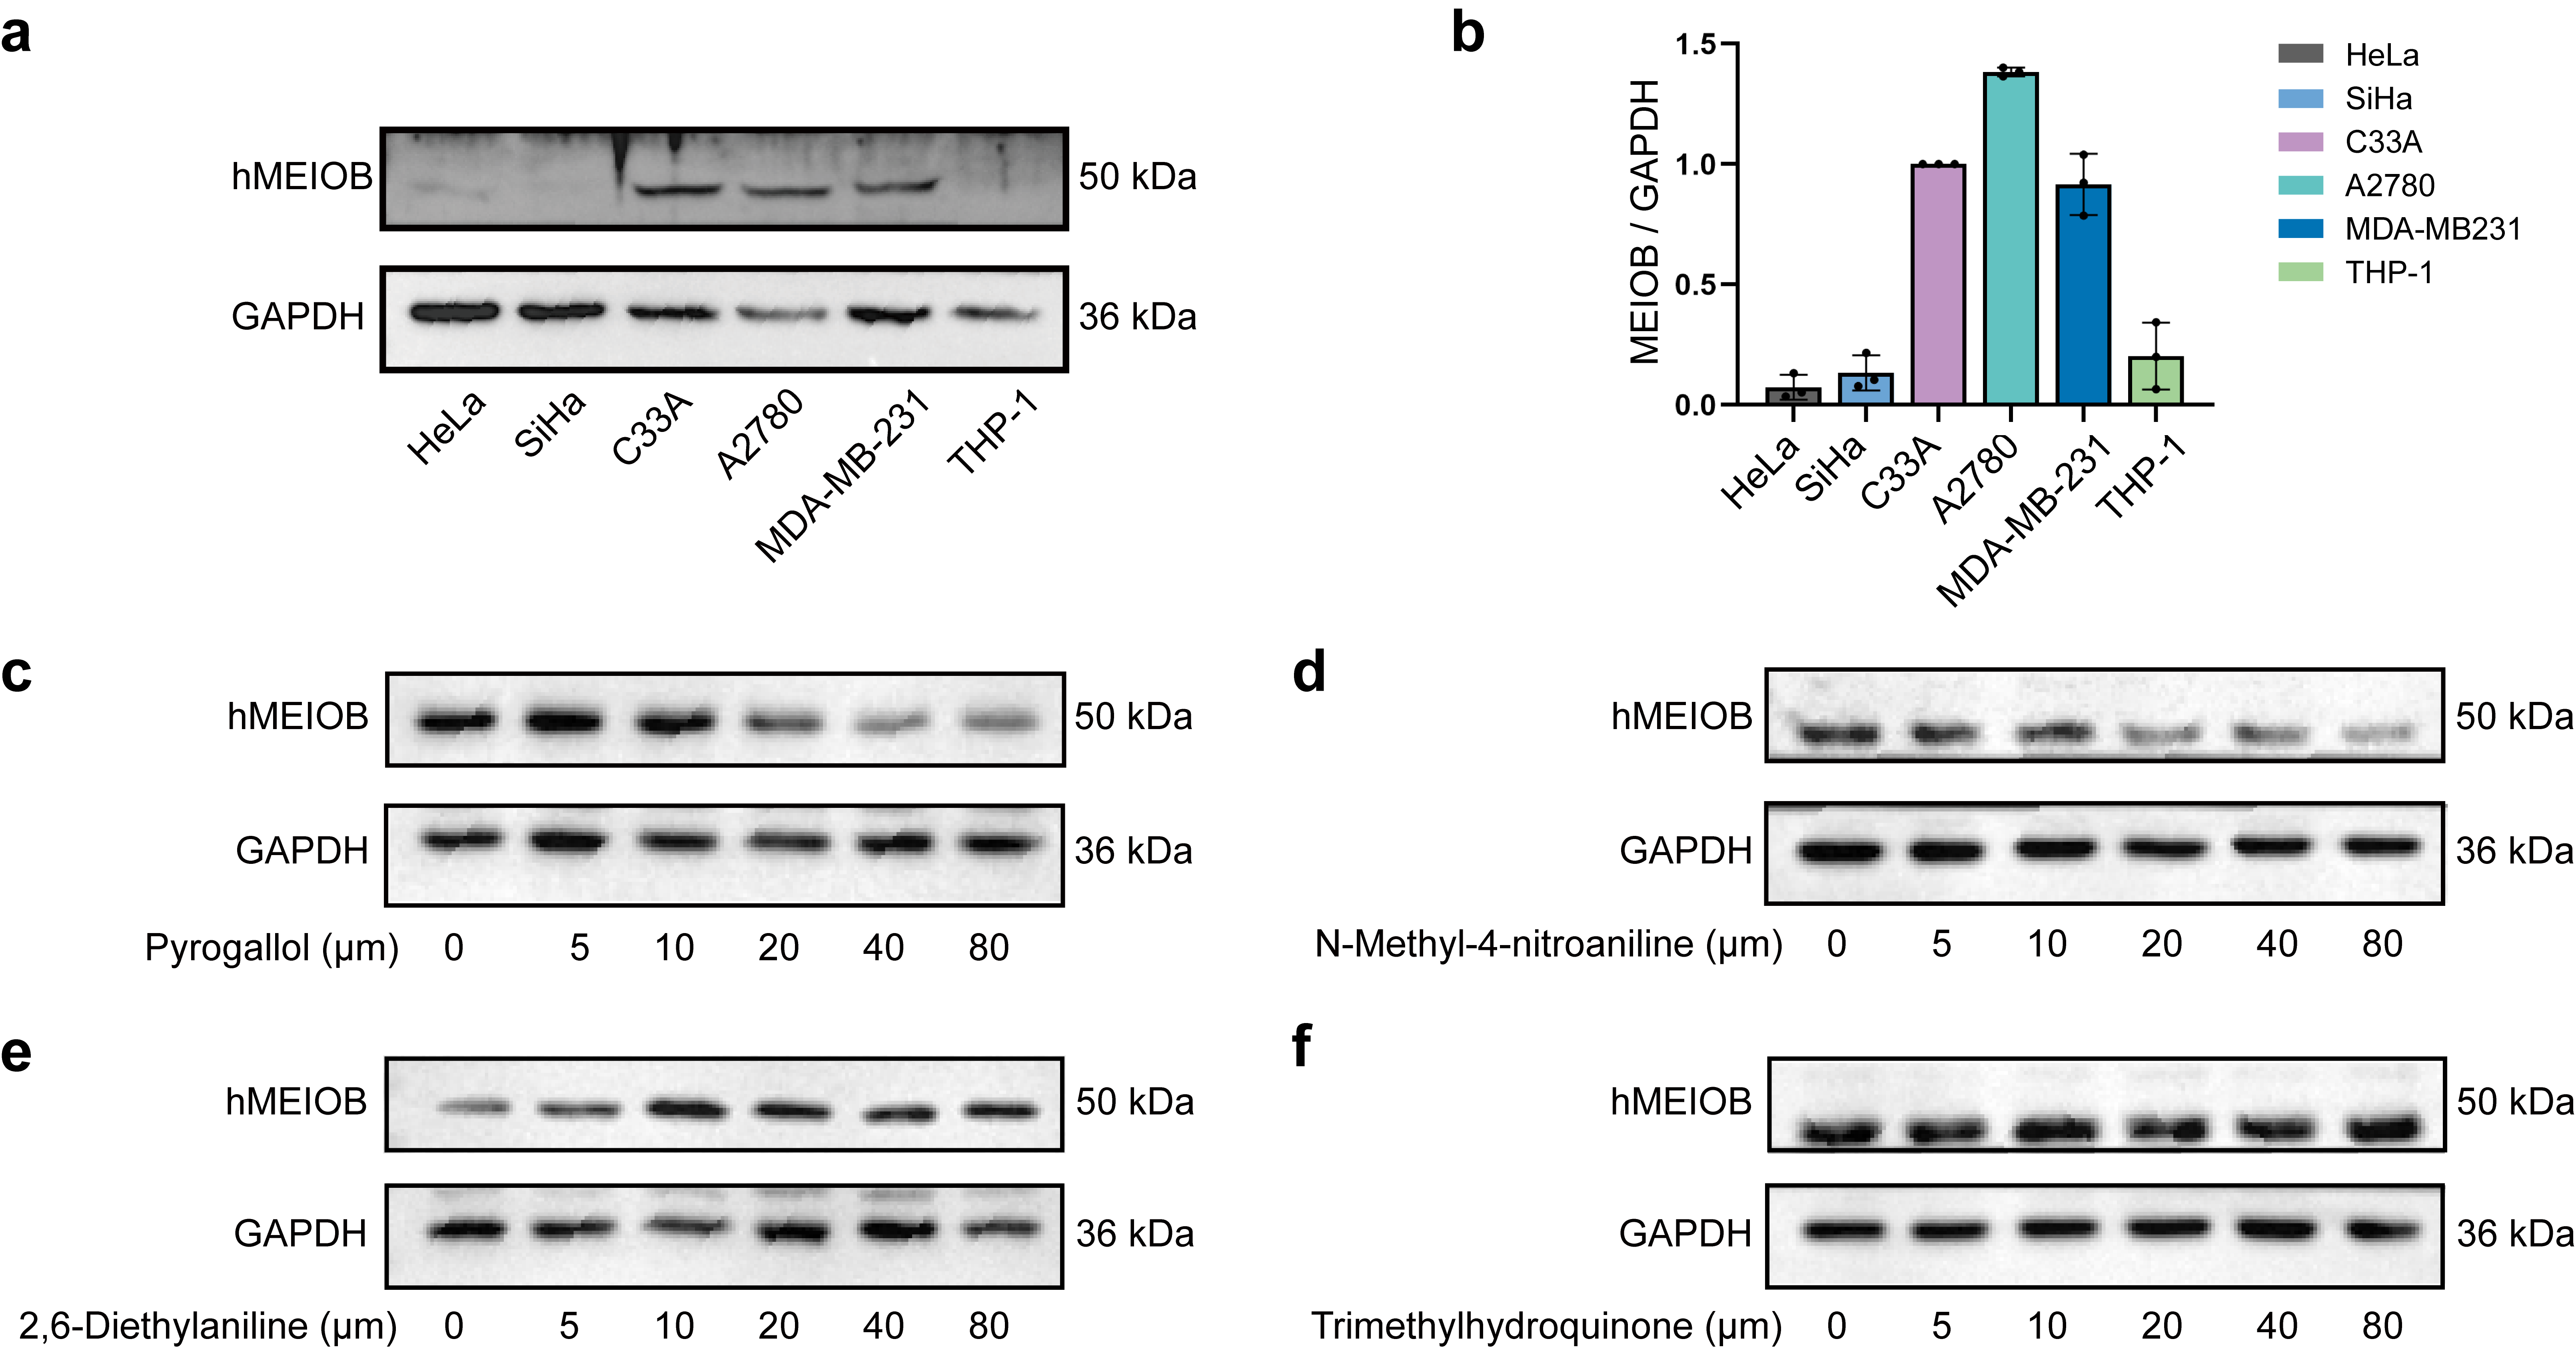
\includegraphics[width=1\linewidth]{pic/Fig 6.png}
%         \caption{\textbf{Small molecules inhibit the expression of MEIOB in C33A cells and affect the cell functions}. \textbf{a} Detect the expression of MEIOB in various tumor cells (HeLa, SiHa, C33A, A2780, MDA-MB-231, THP-1). \textbf{b} Expression levels of MEIOB protein in different tumor cell lines(HeLa, SiHa, C33A, A2780, MDA-MB-231, THP-1). Protein expression levels were quantified by gray values. The relative expression level of MEIOB was normalized using GAPDH as an internal reference (expressed as the MEIOB/GAPDH ratio), and then further normalized to the MEIOB/GAPDH ratio of the C33A group in each experimental set. \textbf{c} The expression level of MEIOB in C33A cells after treatment with pyrogallol for 48 h. \textbf{d} The expression level of MEIOB in C33A cells after treatment with N-methyl-4-nitroaniline for 48 h. \textbf{e} The expression level of MEIOB in C33A cells after treatment with 2,6-diethylaniline for 48 h. \textbf{f} The expression level of MEIOB in C33A cells after treatment with trimethylhydroquinonel for 48 h. Band quantification was normalized to GAPDH. All experiments were independently repeated three times, and the quantitative results were presented as mean±SD.}
%     \label{fig:6}
% \end{figure*}



% \begin{figure*}[ht!]
%     \centering
%     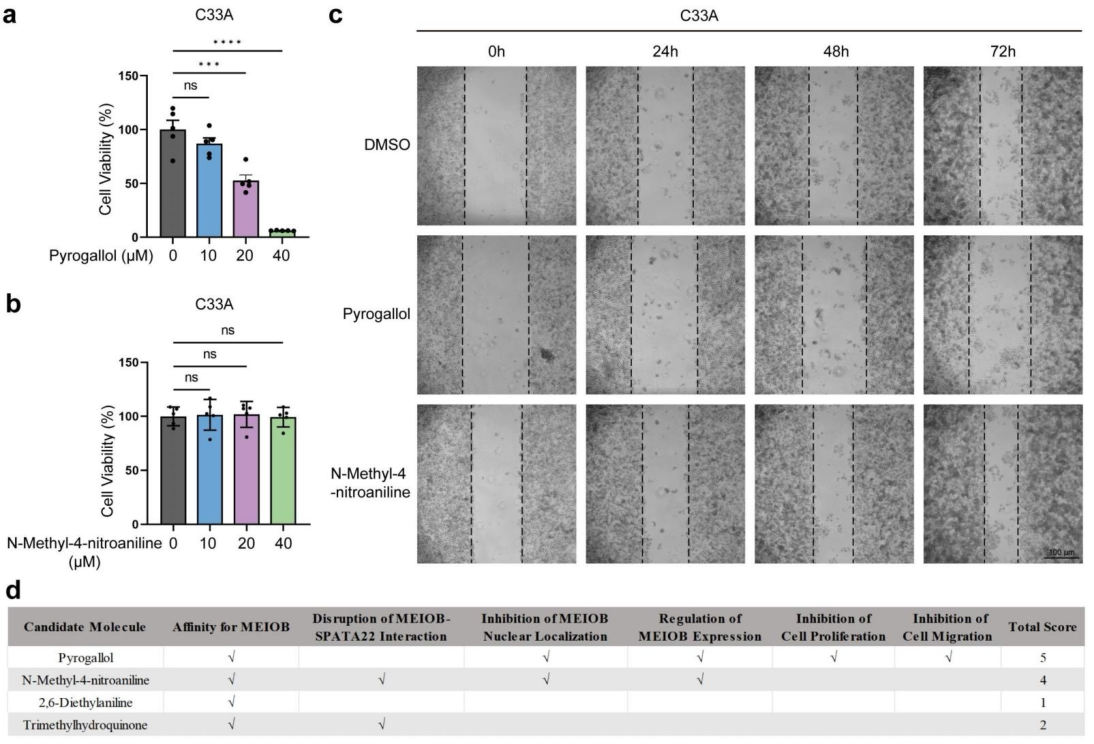
\includegraphics[width=0.8\linewidth]{newpic/fig6.pdf}
%         \caption{\textbf{Small molecules inhibit the cell functions.} \textbf{a} The cell viability of C33A cells after treatment with pyrogallol or N-methyl-4-nitroanilinel for 24 h. n=3/group, ** P  < 0.01, *** P  < 0.001 by two-way ANOVA. All experiments were independently repeated at least three times, and data are shown as the mean$\pm$SD. \textbf{c} The wound-healing assay was employed to assess the impacts of pyrogallol and N-methyl-4-nitroaniline on the migratory capacity of C33A cells. \textbf{d} Scoring of MEIOB-related assays for candidate molecules. Each positive result counted as 1 point. \textcolor{red}{without the b subfigure's caption.}
%         }
%     \label{fig:6}
% \end{figure*}


\subsubsection*{Pyrogallol Inhibits the Proliferation and Migration Abilities of C33A Cells}

Based on the aforementioned experimental data, pyrogallol and N-methyl-4-nitroaniline were shown to inhibit the expression of MEIOB in cervical cancer cells. To understand whether pyrogallol and N-methyl-4-nitroaniline affect the viability of cervical cancer cells, we treated C33A cells with different concentrations of candidate molecules and detected their viability at different times. The CCK-8 assay results showed that the proliferation capacity of C33A cells in the pyrogallol-treated group was significantly inhibited, and the cell survival rate decreased with the increase in the concentration of the candidate molecule (Fig.~\ref{fig:6}f). In contrast, no significant change in cell viability was observed in the N-methyl-4-nitroaniline-treated group (Fig.~\ref{fig:6}h).

Subsequently, we treated C33A cells with pyrogallol and N-methyl-4-nitroaniline and collected images at 0 h, 24 h, 48 h, and 72 h after treatment to observe the effect of candidate molecules on the migration ability of cervical cancer cells. It was found that after treatment with 80 $\mu$M pyrogallol, the migration ability of C33A cells decreased significantly, whereas no obvious change was observed in the migration ability of cells in the N-methyl-4-nitroaniline-treated group (Fig.~\ref{fig:6}i). These results demonstrate that pyrogallol significantly inhibits the proliferation and migration capacities of C33A cells, and this effect is most likely mediated by downregulating MEIOB expression.

Next, we scored the candidate molecules, with the scoring criteria including affinity for MEIOB, regulation of MEIOB expression, disruption of MEIOB-SPATA22 interaction, regulation of MEIOB expression,, inhibition of cell proliferation, and inhibition of cell migration. Each positive test was counted as 1 point. The data showed that pyrogallol exerts the strongest inhibitory effect on MEIOB function, and this effect is likely mediated by disrupting the MEIOB-SPATA22 interaction and inhibiting MEIOB expression (Fig.~\ref{fig:6}j).

% \begin{figure*}
%     \centering
%     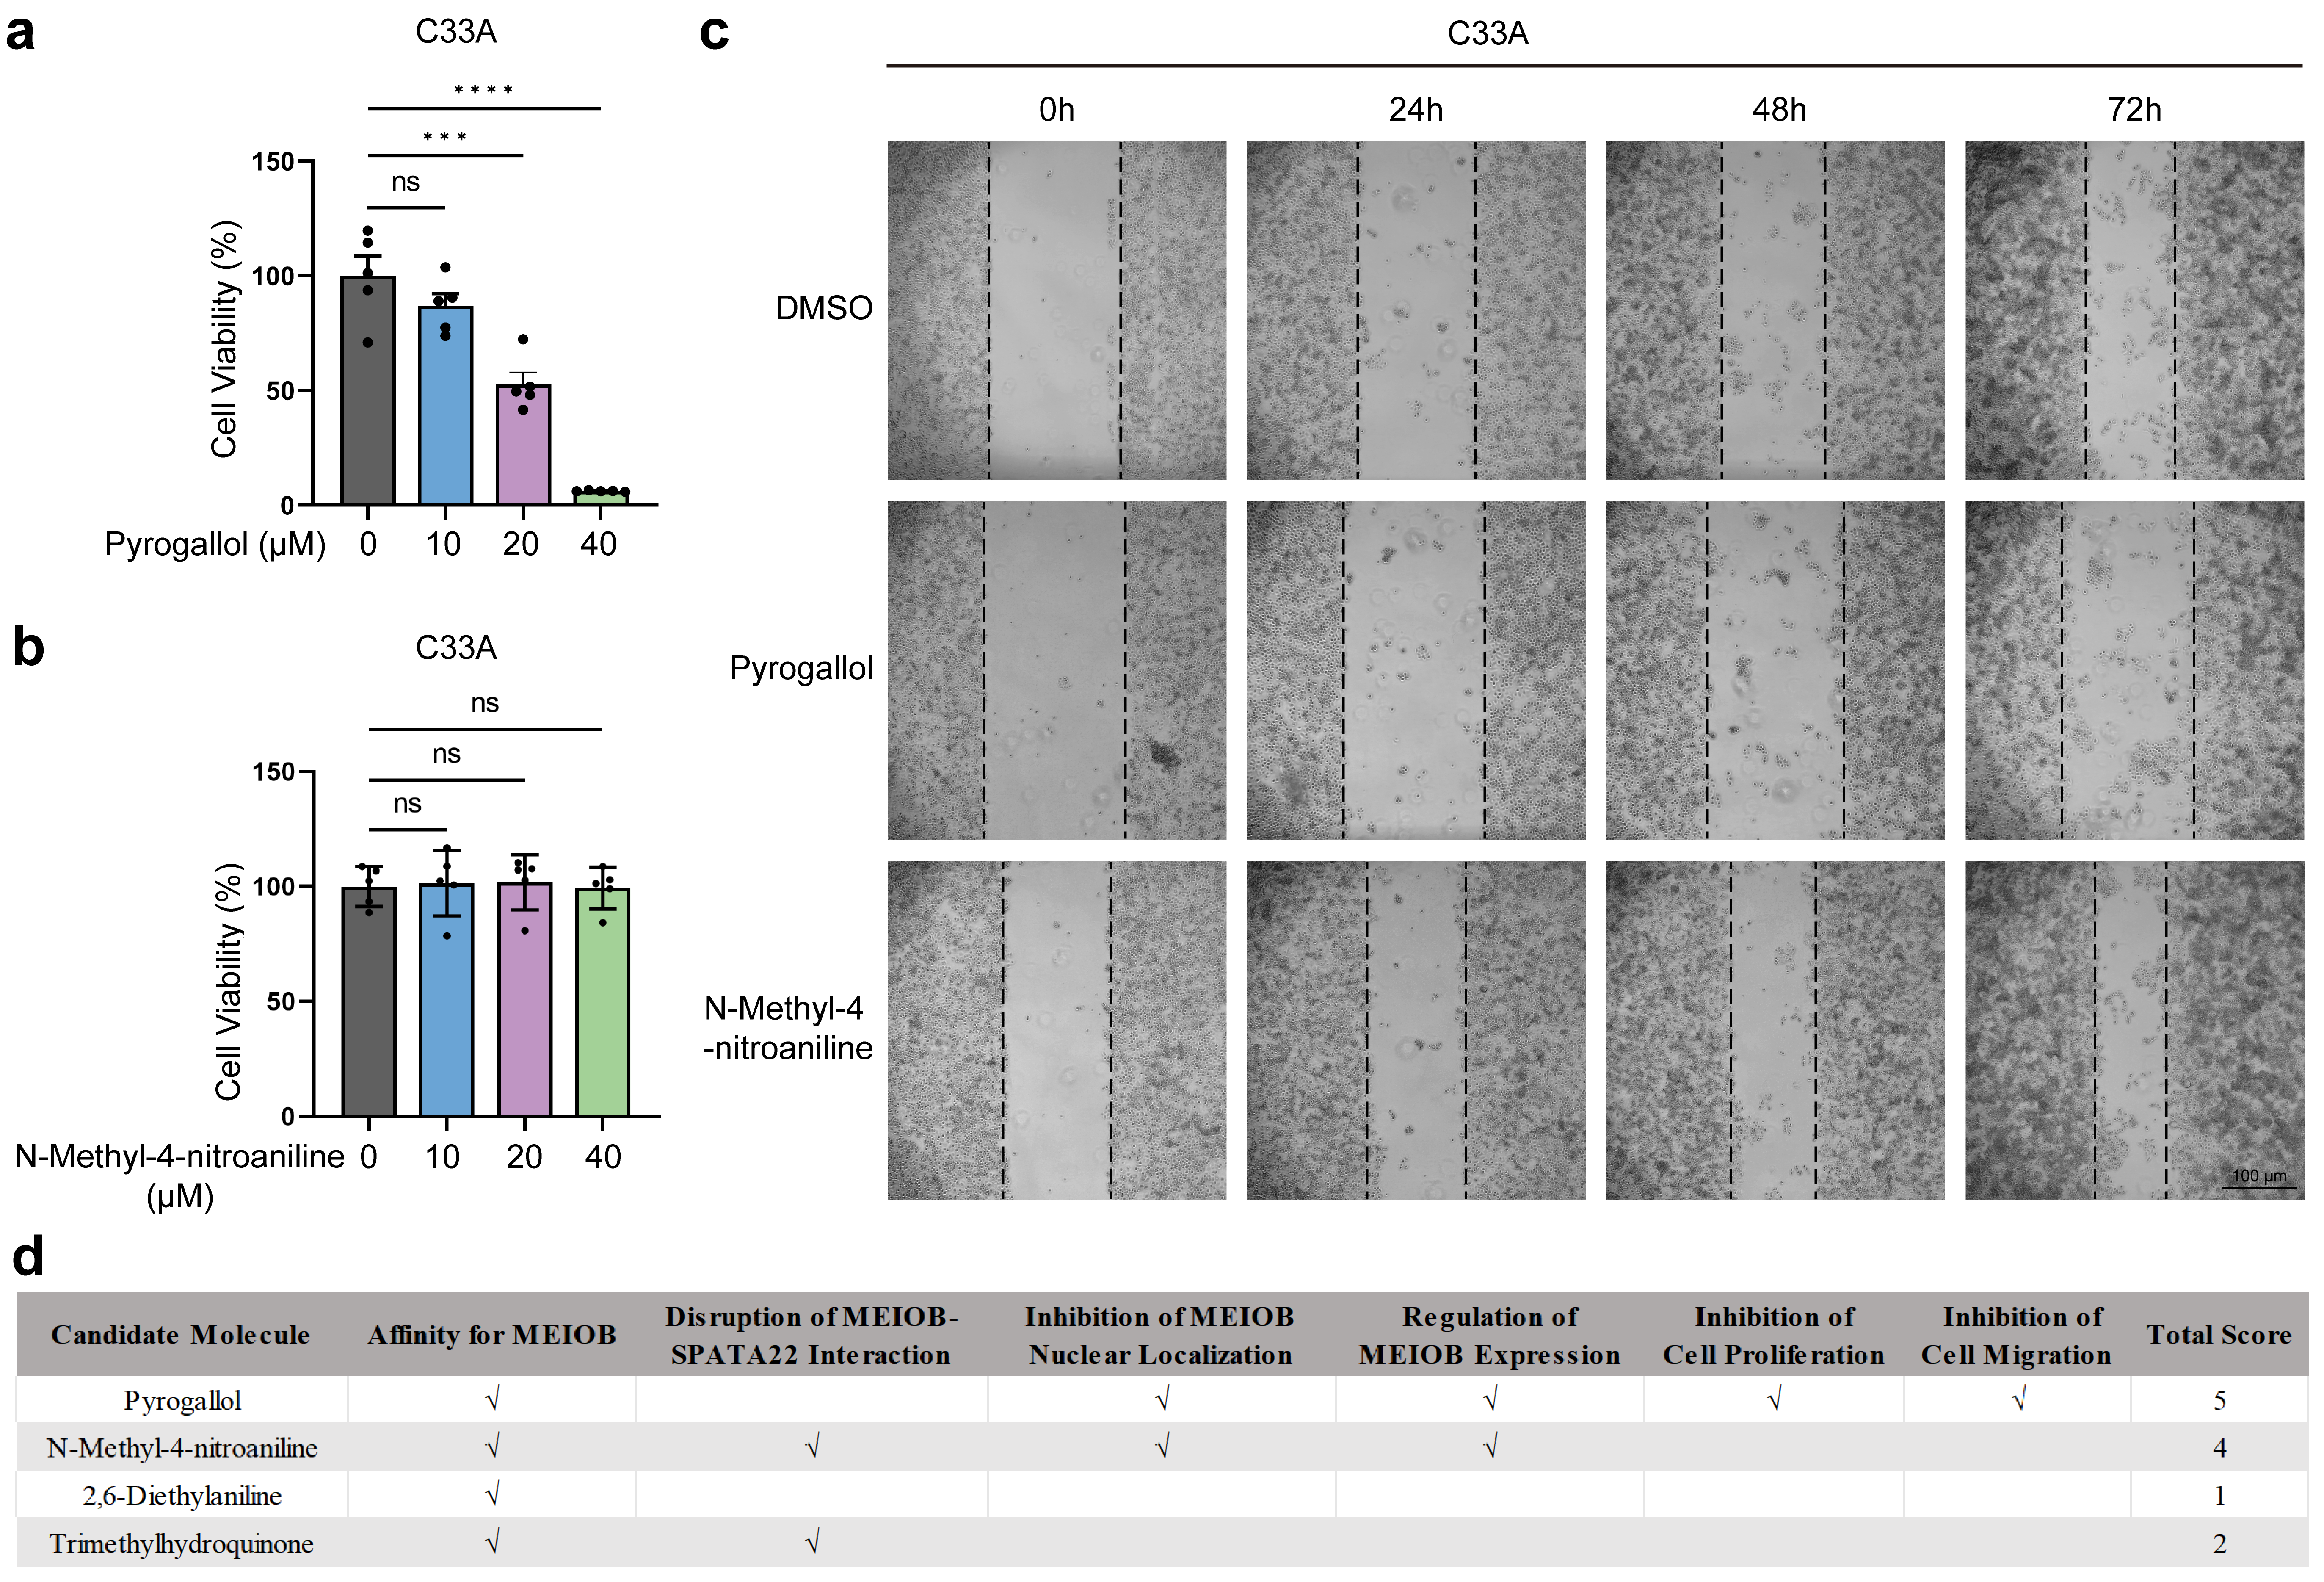
\includegraphics[width=0.8\linewidth]{pic/Fig 7.png}
%         \caption{\textbf{Small molecules inhibit the cell functions}. \textbf{a} The cell viability of C33A cells after treatment with pyrogallol or N-methyl-4-nitroanilinel for 24 h. n=3/group,  $^{\ast\ast}P < 0.01$,  $^{\ast\ast\ast}P < 0.001$ by two-way ANOVA. All experiments were independently repeated at least three times and data are shown as the mean±SD. \textbf{c} The wound-healing assay was employed to assess the impacts of pyrogallol and N-methyl-4-nitroaniline on the migratory capacity of C33A cells. \textbf{d} Scoring of MEIOB-related assays for candidate molecules. Each positive result counted as 1 point.}
%     \label{fig:7}
% \end{figure*}


\section*{Conclusion}
This study presents a multi-stage, multi-model hybrid screening solution for male contraceptive compound screening. By targeting two key proteins, MEIOB and SPATA22, our solution, MMCDS, facilitated the efficient identification of candidate compounds and screened out 4 compounds with micromolar potency. This innovative solution addresses long-standing issues in male contraceptive development, including low screening efficiency and extreme class imbalance (\citealt{54,55,56}). Compared with the current SOTA methods (\citealt{57,58}), MMCDS achieves a 3.80-10.23\% improvement in candidate compound screening accuracy. Overall, this study provides a novel solution for AI-driven screening of male contraceptive compounds. In the face of challenges such as limited data and inconsistent labeling, MMCDS offers a generalizable paradigm that can be extended to small-molecule drug discovery in other therapeutic areas.

% The core strength of MMCDS lies in its synergistic integration of classification and regression models: the classification stage ensures rapid primary filtering, while the regression stage provides refined and quantitative evaluation of compound–target binding affinity. Specifically, a fingerprint-based similarity strategy was employed to optimize sample distribution during classification, mitigating the negative effects of massive inactive molecules on model performance. In the regression stage, contrastive learning and ranking loss were introduced to enhance the model's ability to identify high-potential compounds under data-scarce scenarios. This progressive and hierarchical framework not only improves the robustness and credibility of the entire screening process, but also reduces computational costs and yields a high-confidence candidate pool for downstream wet-lab validation. 


% \section*{Discussion}


% This study presents a multi-stage, multi-model hybrid screening solution for male contraceptive compound screening. By targeting two key proteins, MEIOB and SPATA22, our solution, MMCDS, facilitated the efficient identification of candidate compounds, screened out 4 compounds with micromolar potency. This innovative solution addresses long-standing issues in male contraceptive development, including low screening efficiency and extreme class imbalance (\citealt{54,55,56}). Compared with the current SOTA methods (\citealt{57,58}), MMCDS achieves a 3.80-10.23\% improvement in candidate compound screening accuracy. The core strength of MMCDS lies in its synergistic integration of classification and regression models: the classification stage ensures rapid primary filtering, while the regression stage provides refined and quantitative evaluation of compound–target binding affinity. Specifically, a fingerprint-based similarity strategy was employed to optimize sample distribution during classification, mitigating the negative effects of massive inactive molecules on model performance. In the regression stage, contrastive learning and ranking loss were introduced to enhance the model's ability to identify high-potential compounds under data-scarce scenarios. This progressive and hierarchical framework not only improves the robustness and credibility of the entire screening process, but also reduces computational costs and yields a high-confidence candidate pool for downstream wet-lab validation.

% Most importantly, we successfully validated 4 candidate molecules via BLI assay. Among them, pyrogallol and N-methyl-4-nitroaniline exhibit extremely strong binding affinity, with equilibrium $\text{KD}$ values reaching the 10$^{-7}$ M level, demonstrating excellent potential for clinical translation. The candidate molecules identified in this study impede the interaction between MEIOB and SPATA22 and reduce MEIOB nuclear localization, consistent with our previous finding that SPATA22 is a key protein mediating MEIOB nuclear import (\citealt{10}). However, the specific mechanism of these candidate molecules (including targeted amino acid residues) remains to be further elucidated. Notably, in C33A cells, pyrogallol and N-methyl-4-nitroaniline downregulate MEIOB expression, with pyrogallol significantly inhibiting C33A cell proliferation and migration. This suggests their potential for dual application in male contraception and cancer therapy. Several unresolved questions remain: (1) SPATA22 regulation of MEIOB in tumors and its axis function in oncogenesis remain unclear; (2) Candidate molecules may regulate MEIOB via transcription/translation inhibition or protein interaction interference (mechanism to be explored) (\citealt{18}). Given MEIOB's high tumor expression and role in genome instability, identified inhibitors hold dual contraceptive/anticancer potential, advancing concurrent drug development. Nevertheless, the current work focuses primarily on in vitro functional validation; future investigations in animal models are essential to evaluate in vivo efficacy and safety, paving the way for preclinical development.

% Although these preliminary findings reveal its potential application value in cancer therapy, we recognize that the MMCDS method itself still has several limitations that urgently need improvement. First, due to the limited accuracy of current protein structure prediction tools (\citealt{59,60}), we use features extracted from the primary amino acid sequence. This helps reduce the reliance on 3D structures but also limits the ability to capture dynamic conformations and the detailed geometry of local binding pockets (\citealt{61}). This issue is closely related to the inherent limitations of tools like AlphaFold3 (\citealt{62}). Second, although the KIBA dataset was introduced to increase the diversity of protein targets, the lack of high-quality, target-specific data remains a major barrier (\citealt{63,64}). Public datasets often cover only a small part of the chemical space, and about 70\% of known targets have little or no data on compound binding (\citealt{65}). In addition, inconsistent experimental standards make it hard to compare data across different targets. These factors limit the ability of current methods to fully model complex interaction mechanisms (\citealt{66}).

% Our MMCDS solution still has room for improvement in data collection and integration. The experimental dataset used in this study comprises only 177 samples with precise quantitative values, which may introduce potential data bias.  In future work, we plan to incorporate experimental data from recent studies to retrain the model and enhance the accuracy of drug–target interaction predictions.  Additionally, we will perform structure-based optimization on several promising compounds, such as pyrogallol and N-methyl-4-nitroaniline.

% Overall, this study provides a novel solution for AI-driven male contraceptive compound screening. In the face of challenges such as limited data and inconsistent labeling, MMCDS offers a generalizable paradigm that can be extended to small-molecule drug discovery in other therapeutic areas.


% \clearpage

% \clearpage

% =============================================
% =============================================
% =============================================
% =============================================
% =============================================


% =============================================
% =============================================
% =============================================
% =============================================
% =============================================



\section*{Data availability}

ChemDiv and ChemBridge are both large-scale compound databases, accessible at \url{https://www.chemdiv.com/} and \url{https://chembridge.com/}, respectively. The source data of KIBA dataset used to train and evaluate the model is available at \url{https://tdcommons.ai/multi_pred_tasks/dti/#kiba}. The initial pool of candidate molecules is composed of NCI60(\url{https://dctd.cancer.gov/drug-discovery-development/assays/high-throughput-screening-services/nci60}), CTRP(\url{https://portals.broadinstitute.org/ctrp/}), gCSI(\url{https://pharmacodb.ca/datasets/10}), GDSCv1(\url{https://www.cancerrxgene.org/}), BindingDB(\url{https://tdcommons.ai/multi_pred_tasks/dti/%23bindingdb}), Davis(\url{https://tdcommons.ai/multi_pred_tasks/dti/%23davis}), BioSNAP(\url{https://github.com/peizhenbai/DrugBAN/tree/main/datasets/biosnap}), Human(\url{https://github.com/peizhenbai/DrugBAN/tree/main/datasets/human}), C.elegans(\url{https://github.com/lifanchen-simm/transformerCPI/tree/master/Human%2CC.elegans}), and Lipo, BACE, BBBP, ESOL, HIV, QM7/8/9 available at \url{https://moleculenet.org/datasets-1}. Source data are provided with this paper.



\section*{Code availability}
The source data and codes of DTIAM are available on GitHub at \url{https://github.com/Cello2195/MMCDS}. Rigid docking was performed by Schrödinger (\url{https://www.schrodinger.com}). Preferential binding mode was visualized by Pymol v3.0.3 (\url{https://www.pymol.org/}). RDKit v2023.3.3 (\url{https://www.rdkit.org/}) and ChemDraw v23.1.1 (\url{https://revvitysignals.com/products/research/chemdraw}) were utilized to obtain and visualize the chemical structure from the SMILES. OriginPro 2024b v10.1.5.132 (\url{https://www.originlab.com/}) was used for plotting the data.


\section*{Acknowledgements}

This work was supported in part by the Natural Science Foundation of China (No. 62476203, No. 32270905), Key Project of Traditional Chinese Medicine Joint Fund of Hubei Provincial Natural Science Foundation (No. 2025AFD47), Hubei Province Science and Technology Innovation Plan Project (No. 2025BCB035), the Guangdong Provincial Natural Science Foundation General Project (No. 2025A1515012155). It was also supported by the Natural Science Foundation of Hubei Province - Innovation Group project (No. 2024AFA018), Shenzhen Municipal Science and Technology Innovation Committee (JCYJ20240813111406009), Zhongnan Hospital (ZNLH202206), and Yichun Maternal and Child Health Hospital to Dr. Mengcheng Luo.

\section*{Contributions}

K.L., L.M, and Y.X. contributed equally. \textbf{Y.X.,} X.W., Y.L., M.L., and W.H, conceived and directed the project. All authors contributed substantially to the design and execution of the study, and have reviewed and approved the final manuscript. \textbf{K.L., L.M, and Y.X.} processed the experimental data, performed the analysis, drafted the manuscript and designed the figures.  All contributions have been appropriately acknowledged. The research was conducted in a collaborative and inclusive manner, with equitable involvement of all partners.

\section*{Ethics declarations}

\textbf{Competing interests}. The authors declare no competing interests.


%UNCOMMENT THE BELOW TWO LINES IN CASE YOU NEED AUTHOR YEAR FORMAT.
\bibliographystyle{oup-abbrvnat}
\bibliography{reference}


% ==============================
% \begin{appendices}




% % \bibliography{bib/ref}
% % \bibliographystyle{IEEEtran}
% % \bibliography{refs}



% \section*{Data availability}

% ChemDiv and ChemBridge are both large-scale compound databases, accessible at \url{https://www.chemdiv.com/} and \url{https://chembridge.com/}, respectively. The source data of KIBA dataset used to train and evaluate the model is available at \url{https://tdcommons.ai/multi_pred_tasks/dti/#kiba}. The initial pool of candidate molecules is composed of NCI60(\url{https://dctd.cancer.gov/drug-discovery-development/assays/high-throughput-screening-services/nci60}), CTRP(\url{https://portals.broadinstitute.org/ctrp/}), gCSI(\url{https://pharmacodb.ca/datasets/10}), GDSCv1(\url{https://www.cancerrxgene.org/}), BindingDB(\url{https://tdcommons.ai/multi_pred_tasks/dti/%23bindingdb}), Davis(\url{https://tdcommons.ai/multi_pred_tasks/dti/%23davis}), BioSNAP(\url{https://github.com/peizhenbai/DrugBAN/tree/main/datasets/biosnap}), Human(\url{https://github.com/peizhenbai/DrugBAN/tree/main/datasets/human}), C.elegans(\url{https://github.com/lifanchen-simm/transformerCPI/tree/master/Human%2CC.elegans}), and Lipo, BACE, BBBP, ESOL, HIV, QM7/8/9 available at \url{https://moleculenet.org/datasets-1}. Source data are provided with this paper.



% \section*{Code availability}
% The source data and codes of DTIAM are available on GitHub at \url{https://github.com/Cello2195/MMCDS}. Rigid docking was performed by Schrödinger (\url{https://www.schrodinger.com}). Preferential binding mode was visualized by Pymol v3.0.3 (\url{https://www.pymol.org/}). RDKit v2023.3.3 (\url{https://www.rdkit.org/}) and ChemDraw v23.1.1 (\url{https://revvitysignals.com/products/research/chemdraw}) were utilized to obtain and visualize the chemical structure from the SMILES. OriginPro 2024b v10.1.5.132 (\url{https://www.originlab.com/}) was used for plotting the data.


% \section*{Acknowledgements}

% This work was supported in part by the Natural Science Foundation of China (No. 62476203, No. 32270905), Key Project of Traditional Chinese Medicine Joint Fund of Hubei Provincial Natural Science Foundation (No. 2025AFD47), Hubei Province Science and Technology Innovation Plan Project (No. 2025BCB035), the Guangdong Provincial Natural Science Foundation General Project (No. 2025A1515012155). It was also supported by the Natural Science Foundation of Hubei Province - Innovation Group project (No. 2024AFA018), Shenzhen Municipal Science and Technology Innovation Committee (JCYJ20240813111406009), Zhongnan Hospital (ZNLH202206), and Yichun Maternal and Child Health Hospital to Dr. Mengcheng Luo.

% \section*{Contributions}

% K.L., L.M, and Y.X. contributed equally. \textbf{Y.X.,} X.W., Y.L., M.L., and W.H, conceived and directed the project. All authors contributed substantially to the design and execution of the study, and have reviewed and approved the final manuscript. \textbf{K.L., L.M, and Y.X.} processed the experimental data, performed the analysis, drafted the manuscript and designed the figures.  All contributions have been appropriately acknowledged. The research was conducted in a collaborative and inclusive manner, with equitable involvement of all partners.

% \section*{Ethics declarations}

% \textbf{Competing interests}. The authors declare no competing interests.

% UNCOMMENT THE BELOW TWO LINES IN CASE YOU NEED NUMBERED FORMAT.
% \bibliographystyle{oup-plain}
% \bibliography{reference}




% \begin{figure*}[ht!]
%     \centering
%     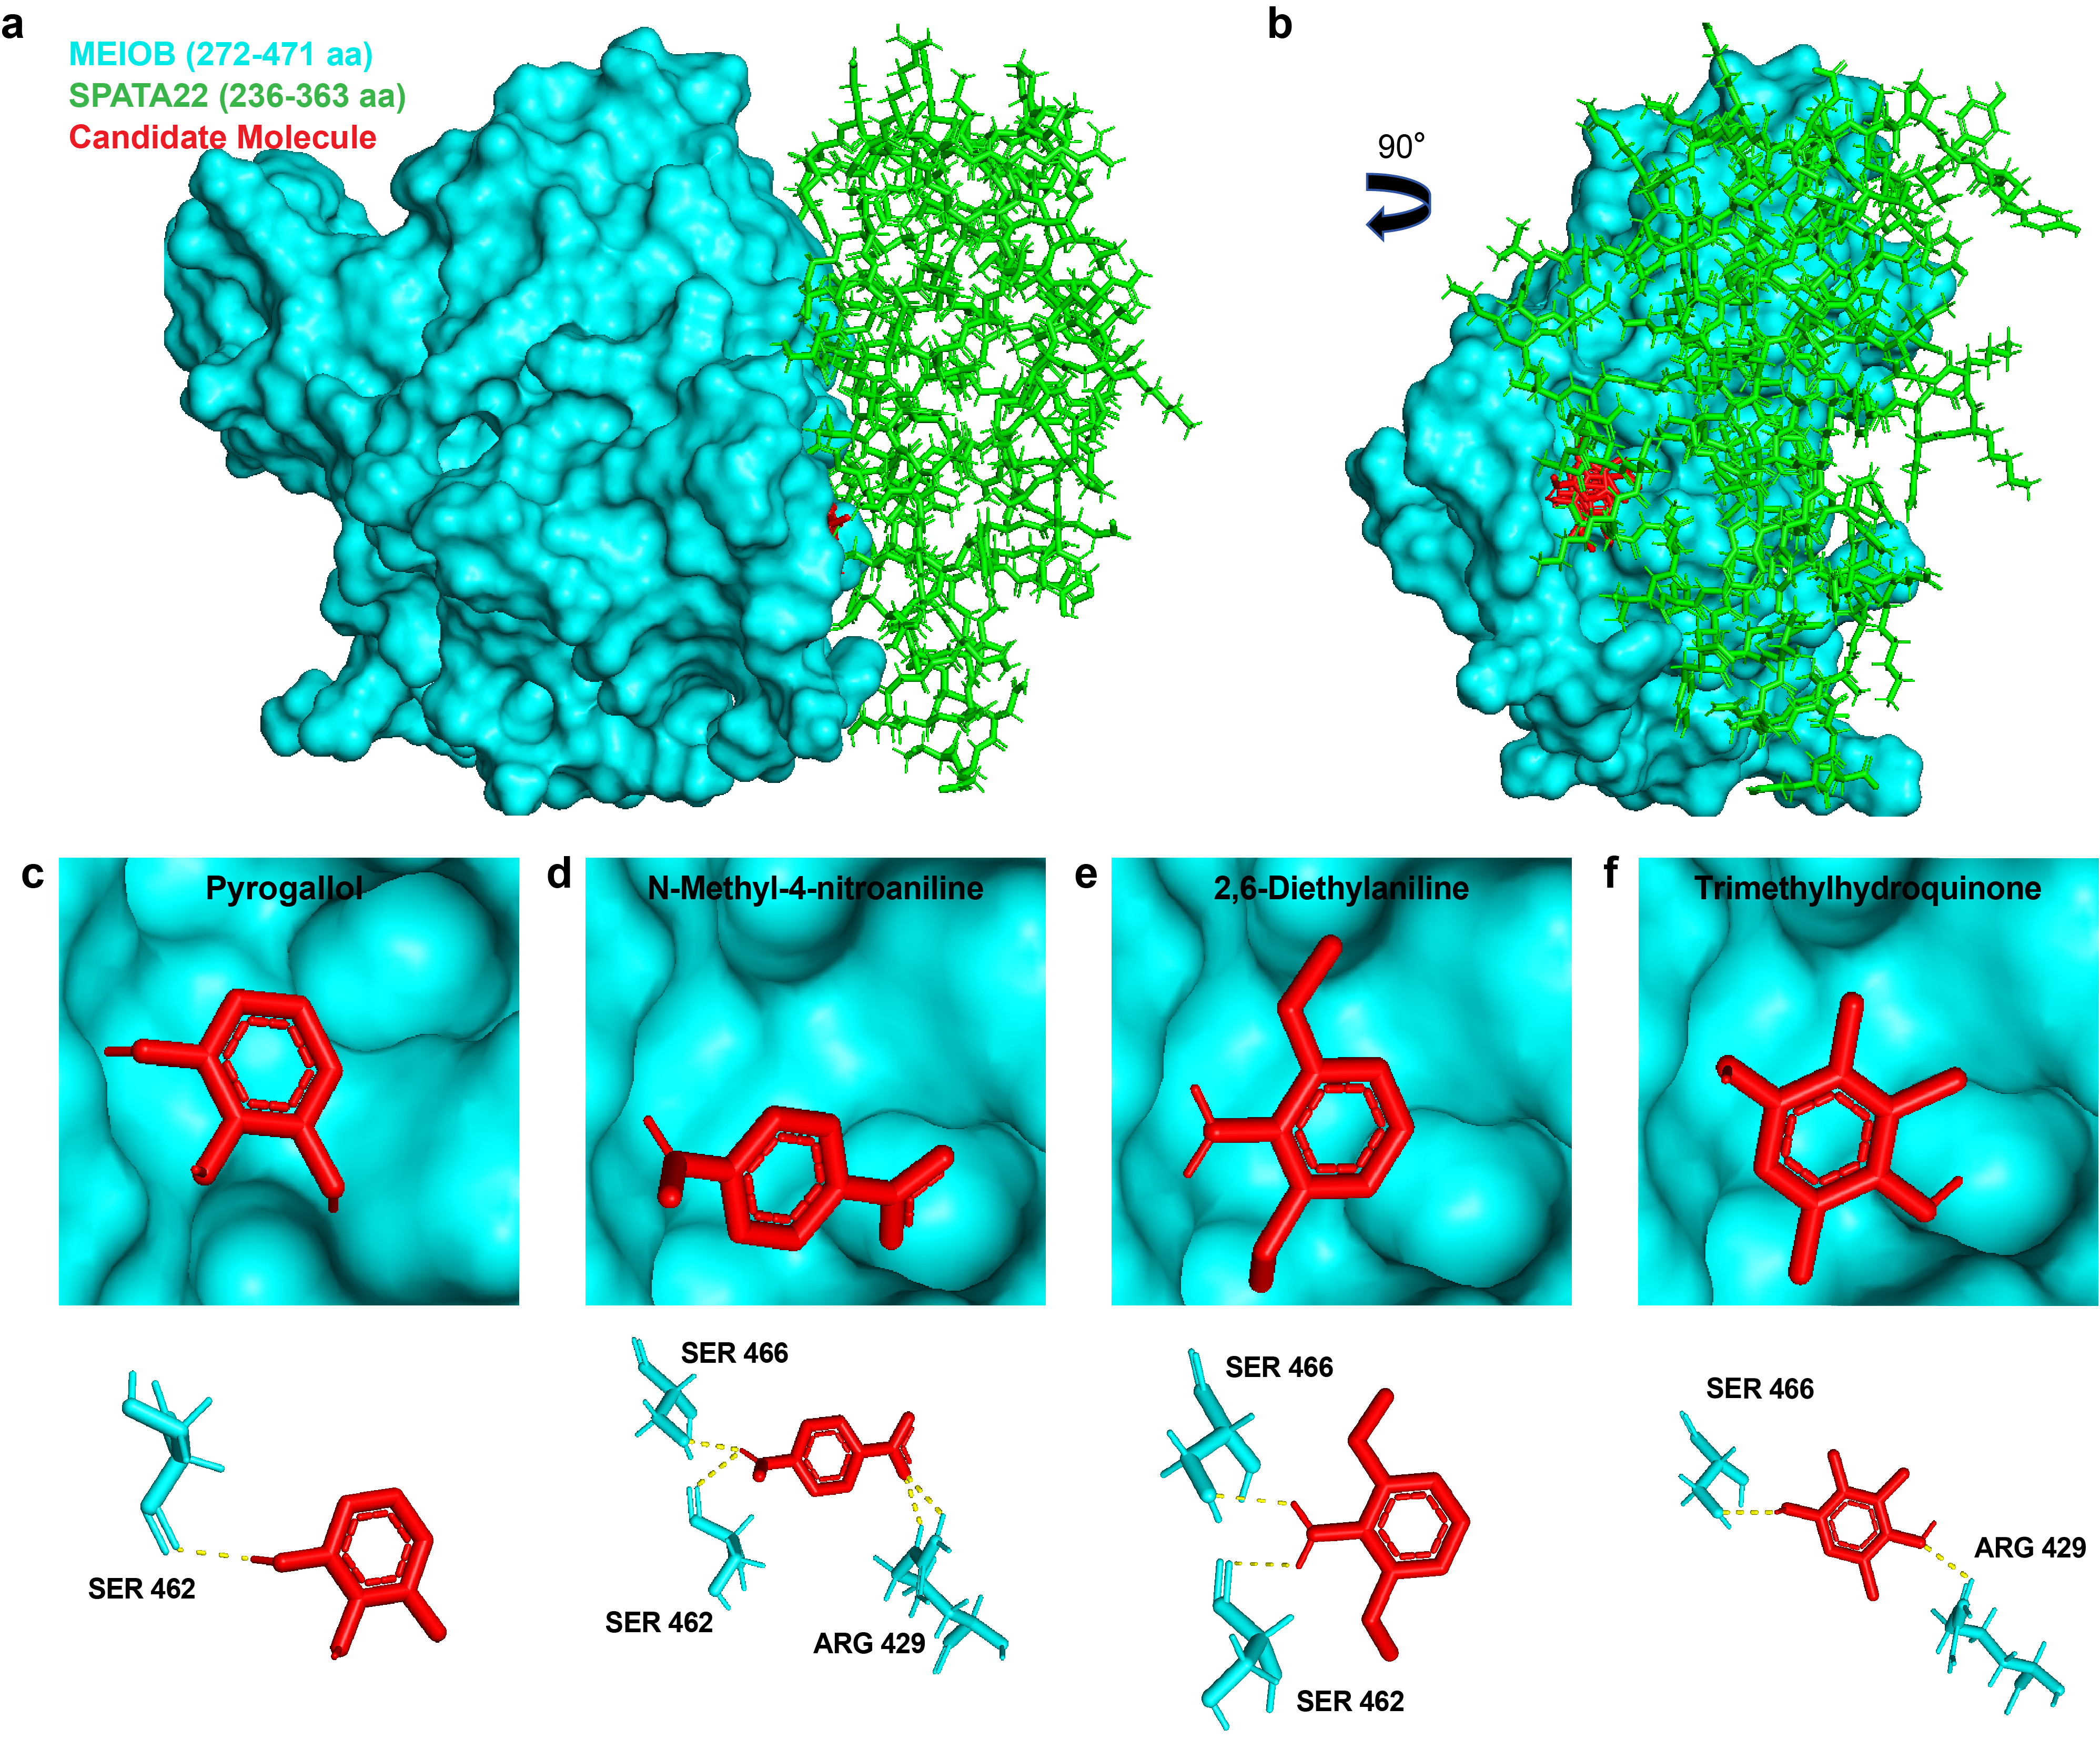
\includegraphics[width=1\linewidth]{pic/Fig S1.png}
%     \caption{\textbf{Molecular docking simulation of small molecule with MEIOB (aa272-471) and SPATA22(aa236-363)}. \textbf{a} Preferential binding mode between compounds and MEIOB according to docking simulation using Pymol software. The amino acid residues involved in interactions are labeled. \textbf{c} Preferential binding mode between pyrogallol and MEIOB. \textbf{d} Preferential binding mode between N-methyl-4-nitroaniline and MEIOB. \textbf{e} Preferential binding mode between 2,6-Diethylaniline and MEIOB. \textbf{f} Preferential binding mode between trimethydroquinone and MEIOB. Cyan: MEIOB; Green: SPATA22; Red: Candidate molecules.}
%     \label{fig:S1}
% \end{figure*}


% \section*{Appendix A: Methods}




% \subsection*{Data collection}

% Previously, we obtained a small molecule library capable of interacting with MEIOB-SPATA22 through high-throughput screening based on the intracellular bimolecular fluorescence complementation (BiFC) assay (\citealt{67}). Derived from Chembridge's Core set library, this compound library contains a total of 177 small molecules, which we classified as effective cases (Supplementary Table 1). Meanwhile, 42,956 samples in the ChemDiv and ChemBridge were viewed as ineffective cases during experiments. Additionally, on account of the fact that the effective cases have different binding abilities with MEIOB-SPATA22, we divided them into 19 true effective cases and 158 false counterparts with a threshold of $-4.2$ based on the distribution of effective cases.


% \subsection*{Data Preprocessing}

% In our experimental dataset, the number of confirmed positive samples (with specific reaction values) is substantially outnumbered by negative samples, resulting in a severe class imbalance that poses significant challenges for training effective classification or regression models directly. Therefore, during the screening stage for potentially effective molecules, we employ molecular fingerprint similarity to select the top k most similar negative samples for each positive sample. By maintaining a controlled positive-to-negative ratio during training, the model achieves more robust boundary discrimination.

% Let the set of positive samples be $\text{D}_{\text{pos}}$ and the set of negative samples be $\text{D}_{\text{neg}}$. We define a similarity function $\text{SimFinger}(\cdot,\cdot)$ to compute the similarity between a positive sample $\text{D}_{\text{pos}}$ and a negative sample $\text{D}_{\text{neg}}$:
% \begin{equation}
% S(\text{D}_{\text{pos}}, \text{D}_{\text{neg}}) = \text{SimFinger}(F_{\text{pos}}, F_{\text{neg}})
% \end{equation}
% where $F_{\text{pos}}$ and $F_{\text{neg}}$ are the molecular fingerprint feature vectors of the positive and negative samples, respectively. The top $k$ negative samples are selected as follows:
% \begin{equation}
% N_k(p) = \{n \in N \,|\, S(p, n) \text{ is top } k \text{ for } p\}
% \end{equation}

% % 将177个有反应数值的数据整合到广泛使用的KIBA数据集中来增强数据集，并将所有测量值映射到合适的数值范围内。
% During the data preprocessing for the ranking phase, there are 177 samples with regression numerical labels (\citealt{67}). Due to the limited sample size, we integrate these 177 response-valued data points into the widely used KIBA dataset to enhance the training data. All measured values are mapped to an appropriate numerical range through linear transformation.

% Let $x_{\text{orig}} \in [a,b]$ represent the original values from our 177 samples, and $y \in [c,d]$ denote the KIBA score range. The linear mapping function is formulated as:
% \begin{equation}
% y = c + \left( \frac{x_{\text{orig}} - a}{b - a} \right) \times (d - c)
% \end{equation}

% This normalization ensures that the original measurements maintain their relative distribution while being aligned with the KIBA dataset's scale.


% \subsection*{Cell culture}

% HeLa, SiHa, MDA-MB-231, A2780, THP-1 and HEK 293T cells were purchased from American Type Culture Collection (ATCC). C33A cells were purchased from Wuhan Pusai Biotechnology Co., Ltd. Cells were cultured in DMEM (BasalMedia Technologies), MEM (Gibco) or RIPA-1640 (Gibco) supplemented with 10\% fetal bovine serum (FBS; AusGeneX) and 100 U/mL penicillin and streptomycin in a humidified 5\% CO$_2$ atmosphere. 


% \subsection*{Protein expression and purification}
% The full-length human MEIOB sequence was codon-optimized by using the Integrated DNA technologies\footnote{https://sg.idtdna.com/pages/} and synthesized by Sangon Biotech. The optimized full-length human MEIOB sequence was inserted into the \textit{Nde}I/\textit{Xho}I restriction sites of the pET-42b(+) vector (Addgene) with 8×His-Tag to construct the pET-42b-hMEIOB-8×His-Tag vector. DNA fragments encoding the CopGFP and mCherry tags were amplified from vectors pCDH-EF1-CopGFP (Addgene) and pCDH-EF1a-eFFly mCherry (Addgene), and then inserted into the \textit{Xho}I/\textit{Xba}I restriction sites of the pcDNA3.1(+) vector (Addgene) to generate pcDNA3.1-CopGFP-C and pcDNA3.1-mCherry-C. The optimized full-length human MEIOB and SPATA22 fragments were inserted into the \textit{Nhe}I/\textit{Xho}I sites of pcDNA3.1-CopGFP-C or pcDNA3.1-mCherry-C. The vectors were constructed and extracted with an EndoFree Mini Plasmid Kit II (TIANGEN). The purified plasmid was transfected into HEK 293T cells with LipofectamineTM 2000 Transfection Reagent (Thermo Fisher). After 8 h, candidate drugs prepared in low-serum medium were added, and the culture was continued for another 48 h. Subsequently, the samples were mounted with mounting medium containing DAPI, followed by observation and photography under the fluorescence microscope (ApoTome.2; ZEISS).

% \subsection*{Protein expression and purification}

% The plasmids pET-42b-hMEIOB-8×His-Tag were transformed into the bacterial strain E. coli BL21 for protein production. A single colony of bacteria from each transformation was selected, inoculated in liquid LB medium (50 $\mu$g/mL kanamycin), and incubated for 6-8 h at 37°C while shaken at 220 rpm. When the OD600 value of the bacterial culture reached 0.6-0.8, IPTG was added to the culture medium at a final concentration of 0.24 mg/mL and the bacteria were grown at 16°C for another 16 h. The bacteria cells were harvested by centrifugation at 5000 × g for 10 min at 4°C. The cell pellet was subjected to high pressure disruption at a pressure of 600 kPa for 8 min at 4°C in lysis buffer (50 mM NaH2PO4, 300 mM NaCl, PH 8.0), and the mixture was centrifuged at 10,000 × g for 10 min at 4°C. Appropriately pre-treated Ni-NTA beads 6FF (Smart-lifesciences) were added in suitable amounts to the supernatant. The mixture was then incubated with a slow rotation at 4°C for 2 h. After that, the mixture was passed through a column. Imidazole (50, 60, 70, 80, 90, 100 mM) was used to remove impurities in a gradient manner. Finally, elution buffer (50 mM NaH$_2$PO$_4$, 300 mM NaCl, 500 mM imidazole, PH 8.0) was added for elution. The purified protein was concentrated using a 10 kDa ultrafiltration centrifugal tube (Millipore). Protein purity was determined by SDS-PAGE, and protein concentration was measured using the BCA Protein Assay Kit (Biosharp).


% \subsection*{Bio-layer Interferometry (BLI)}

% MEIOB's binding to candidate molecules was measured by bio-layer interferometry (BLI) using Octet RED96 systems (fortéBIO). The purified soluble protein with His-Tag was used for analysis. The concentration of the protein was adjusted to 10 $\mu$g/mL using the working buffer (0.02\% Tween20-0.1\% BSA-PBS). The candidate molecules were dissolved in DMSO and their concentrations were adjusted with the working buffer (5000, 2500, 1250, 625, 312.5, 156, 78, 0 nM). 200 $\mu$L of the protein sample and the candidate molecules were added to a 96 - well sample plate, and the binding between them was analyzed by using NTA biosensors (fortéBIO) in the analytical instrument. The method was defined with five steps: Baseline, Loading, Baseline, Association and Dissociation. Data were acquired (kinetics mode) and analyzed using the Data acquisition software v9.0 or Data Analysis software v9.0 (fortéBIO). In addition, the data were exported as a Microsoft Excel file to generate fitted curves. The association and dissociation were calculated based on the response amplitude (wavelength shift in nm) obtained within the time when the sample reached equilibrium. The equilibrium dissociation constant ($\text{KD}$) is determined by the concentration ($\text{Conc.}$) of the small-molecule drug and the signal ($R_{max}$) obtained when all the proteins are occupied by the small-molecule drug. $R_{max}$ is deduced by plotting $\text{Req}$ against the concentration. The concentration at which 50\% of $R_{max}$ is reached is the $KD$ value.

% \begin{eqnarray}
% \text{Req} & = & R_{max} \times  \frac{\text{Conc.}}{\text{KD} + \text{Conc.}} 
% \end{eqnarray}


% \subsection*{Co-immunoprecipitation}
% Cells were lysed using IP lysis buffer(Tris 20 mM, NaCl 140 mM, 2 mM EDTA, 1\%NP-40, PH 7.5). The samples were divided into three tubes: the experimental tube, the IgG tube, and the Input tube. 5×Loading Buffer was added to the Input tube, which was then placed in a 100°C metal bath for 10 minutes and stored at -20°C. For the experimental tube and IgG tube, 3 $\mu$g of anti-mCherry antibody (68088-1-Ig, Proteintech) or Mouse Control IgG (AC011, ABclonal) was added, followed by rotation on a turntable at 4°C overnight. On the next day, 25 $\mu$L of protein A/G magnetic beads (MedChemExpress) were added to the samples, and the mixture was incubated with rotation at 4°C for 2 h. The magnetic beads were washed with PBS buffer, after which the samples were placed on a magnetic rack to separate the magnetic beads. An appropriate amount of 1×Loading buffer was added to the magnetic beads, which were then placed in a 100°C metal bath for 10 min, followed by WB analysis.

% \subsection*{Western Blot Analysis}
% Cells were lysed using RIPA buffer (Tris 20 mM, NaCl 150 mM, KCl 20 mM, MgCl$_2$ 1.5 mM, glycerol 10\%, Triton X‐100 1\%, PH 7.5), and the protein concentration was measured by BCA protein assay kit (Biosharp). Equal amounts of proteins were separated by 12\% sodium dodecyl sulfate‐polyacrylamide gel electrophoresis and were transferred onto polyvinylidene fluoride (PVDF) membranes. The membrane was then blocked with 5\% skimmed milk for 2 h at RT. Primary antibodies including anti-MEIOB (The production of this antibody was mentioned in our previous article (\citealt{6}), and anti-GAPDH (10494-1-AP, Proteintech) antibodies were diluted in Blocking buffer and incubated with PVDF membrane at 4°C overnight. The next day, the membrane was incubated with goat anti-mouse/anti-rabbit secondary antibodies (AS003, AS014, ABclonal) for 1.5 h at room temperature. The target proteins were finally detected using standard WB protocols and visualized using the West ECL Illuminating Liquid (Syngene). 

% \subsection*{CCK-8 Assay}
% The cell proliferation was performed by a SuperKine™ Maximum Sensitivity Cell Counting Kit-8 (Abbkine) assay. C33A cells (1×10$^{4}$ cells) were seeded in 96-well plates and incubated in sterile DMEM with different concentrations of small-molecule drugs (0, 10, 20, 40 $\mu$M) . At specific time points (0, 24, 48, 72, 96 h) , 10 $\mu$L of CCK-8 working solution was added into each well and incubated at 37°C for 2 h. The absorbance at 450 nm was detected using the Sense Microplate Reader (Hidex). The experiment was repeated three times.

% \subsection*{Wound-healing Assay}
% C33A cells (2×10$^{5}$ cells) were cultured in 6-well plates. When the cells were grown to 90\% confluence, the wound was formed by scratching with a 200 $\mu$L pipette tip. Then, the cells were treated with a small-molecule drug at a concentration of 80 $\mu$M. The wound width was measured and captured by microscopy (ApoTome.2; ZEISS).

% \subsection*{Molecular modeling}
% Protein structure information was visualized using PyMOL (version 3.0.3) software (\citealt{68}). The coordinates of the MEIOB (aa272-471) and SPATA22(aa236-363) were generated based on the AlphaFold-predicted structure (\citealt{69}).

% \subsection*{Quantification and statistical analysis}
% Sequence alignment and sequence analysis were carried out using the SnapGene 6.0 software. Statistical analyses were performed using the software GraphPad Prism (version 9.3). For the comparison of data between two groups, an unpaired t-test was used for the analysis of significant differences; for the comparison of data among multiple groups, one-way analysis of variance (One-Way ANOVA) or two-way analysis of variance (two-way ANOVA) were adopted. All error bars denote the mean ± SD. The difference between the various data were considered significant when the \textit{P} value was less than 0.05 ($^{\ast}$), 0.01 ($^{\ast\ast}$) or 0.001 ($^{\ast\ast\ast}$). All results shown in the study are representative of at least three independent experiments with similar results.






% \end{appendices}



\end{document}
